% !TeX root = RJwrapper.tex
\title{A Hexagon Tile Map Algorithm for Displaying Spatial Data}
\author{by Stephanie Kobakian and Dianne Cook}

\maketitle

\abstract{%
This algorithm creates a tessellated hexagon display to represent a set
of the spatial polygons. It allocates these hexagon in a manner that
preserves the spatial relationship of the geographic units. The
algorithm creates a display that showcases spatial distributions, by
emphasising the small geographical regions that are often difficult to
locate on geographic maps. Spatial distributions have been presented on
alternative representations of geography for many years. In modern
times, interactivity and animation have begun to play a larger role, as
alternative representations have been popularised by online news sites,
and atlas websites with a focus on public consumption. Applications are
increasingly widespread, especially in the areas of disease mapping, and
election results.
}

\hypertarget{introduction}{%
\subsection{Introduction}\label{introduction}}

Many cancer atlases present geospatial cancer data on a choropleth map
display. The Australian Cancer Atlas \citep{TACA} is a recent addition
to the many cancer atlas maps worldwide. The ground-breaking atlas for
Australia presents a central map that shows the landmass overlaid with
administrative boundaries. This choropleth display can highlight the
geographic patterns in geospatially related cancer statistics
\citep{SAMGIS}.

In many countries, residents are increasingly gathering to live in urban
areas around major cities \citep{ACTUC}. The creation of approximately
equal population areas results in dramatically different square meterage
of the administrative geographic units, such as states or electorates.
The units are filled with colour to represent the value of the statistic
for each unit \citep{EI}. This can lead to unequal emphasis on the
statistical value of each of the geographic units. This allows
choropleth map displays to misrepresent the spatial distributions of
human related statistics due to area-size bias \citep{BCM}. Figure
\ref{fig:melanoma-geo} is a choropleth map that uses colour to display
the estimated Standardised Incidence Ratios (SIRs) of melanoma cancer
for males for each of the Statistical Areas at Level 2 (SA2) used by the
Australian Bureau of Statistics \citeyearpar{abs2011}. The Australian
choropleth map display draws attention to the expanse of light blue
areas across the rural communities in all states. The SA2s around Hobart
stand out as more orange and red. To create this choropleth map the SA2
polygons for 2011 from the Australian Bureau of Statistics.

The solutions to this visualisation problem begin with the geography.
Alternative maps shift the focus from land area and shape, to the value
of the statistics in a group of areas \citep{ACCAC}. Different styles of
cartograms apply transformations to the geographic areas, to highlight
the values of the value of the statistic of interest. These displays
result in a distortion of the map space to represent differences in the
statistic across the areas \citep{ACCAC} as the statistic of interest is
used to determine the cartogram layout.

\begin{figure}[h]
\centering
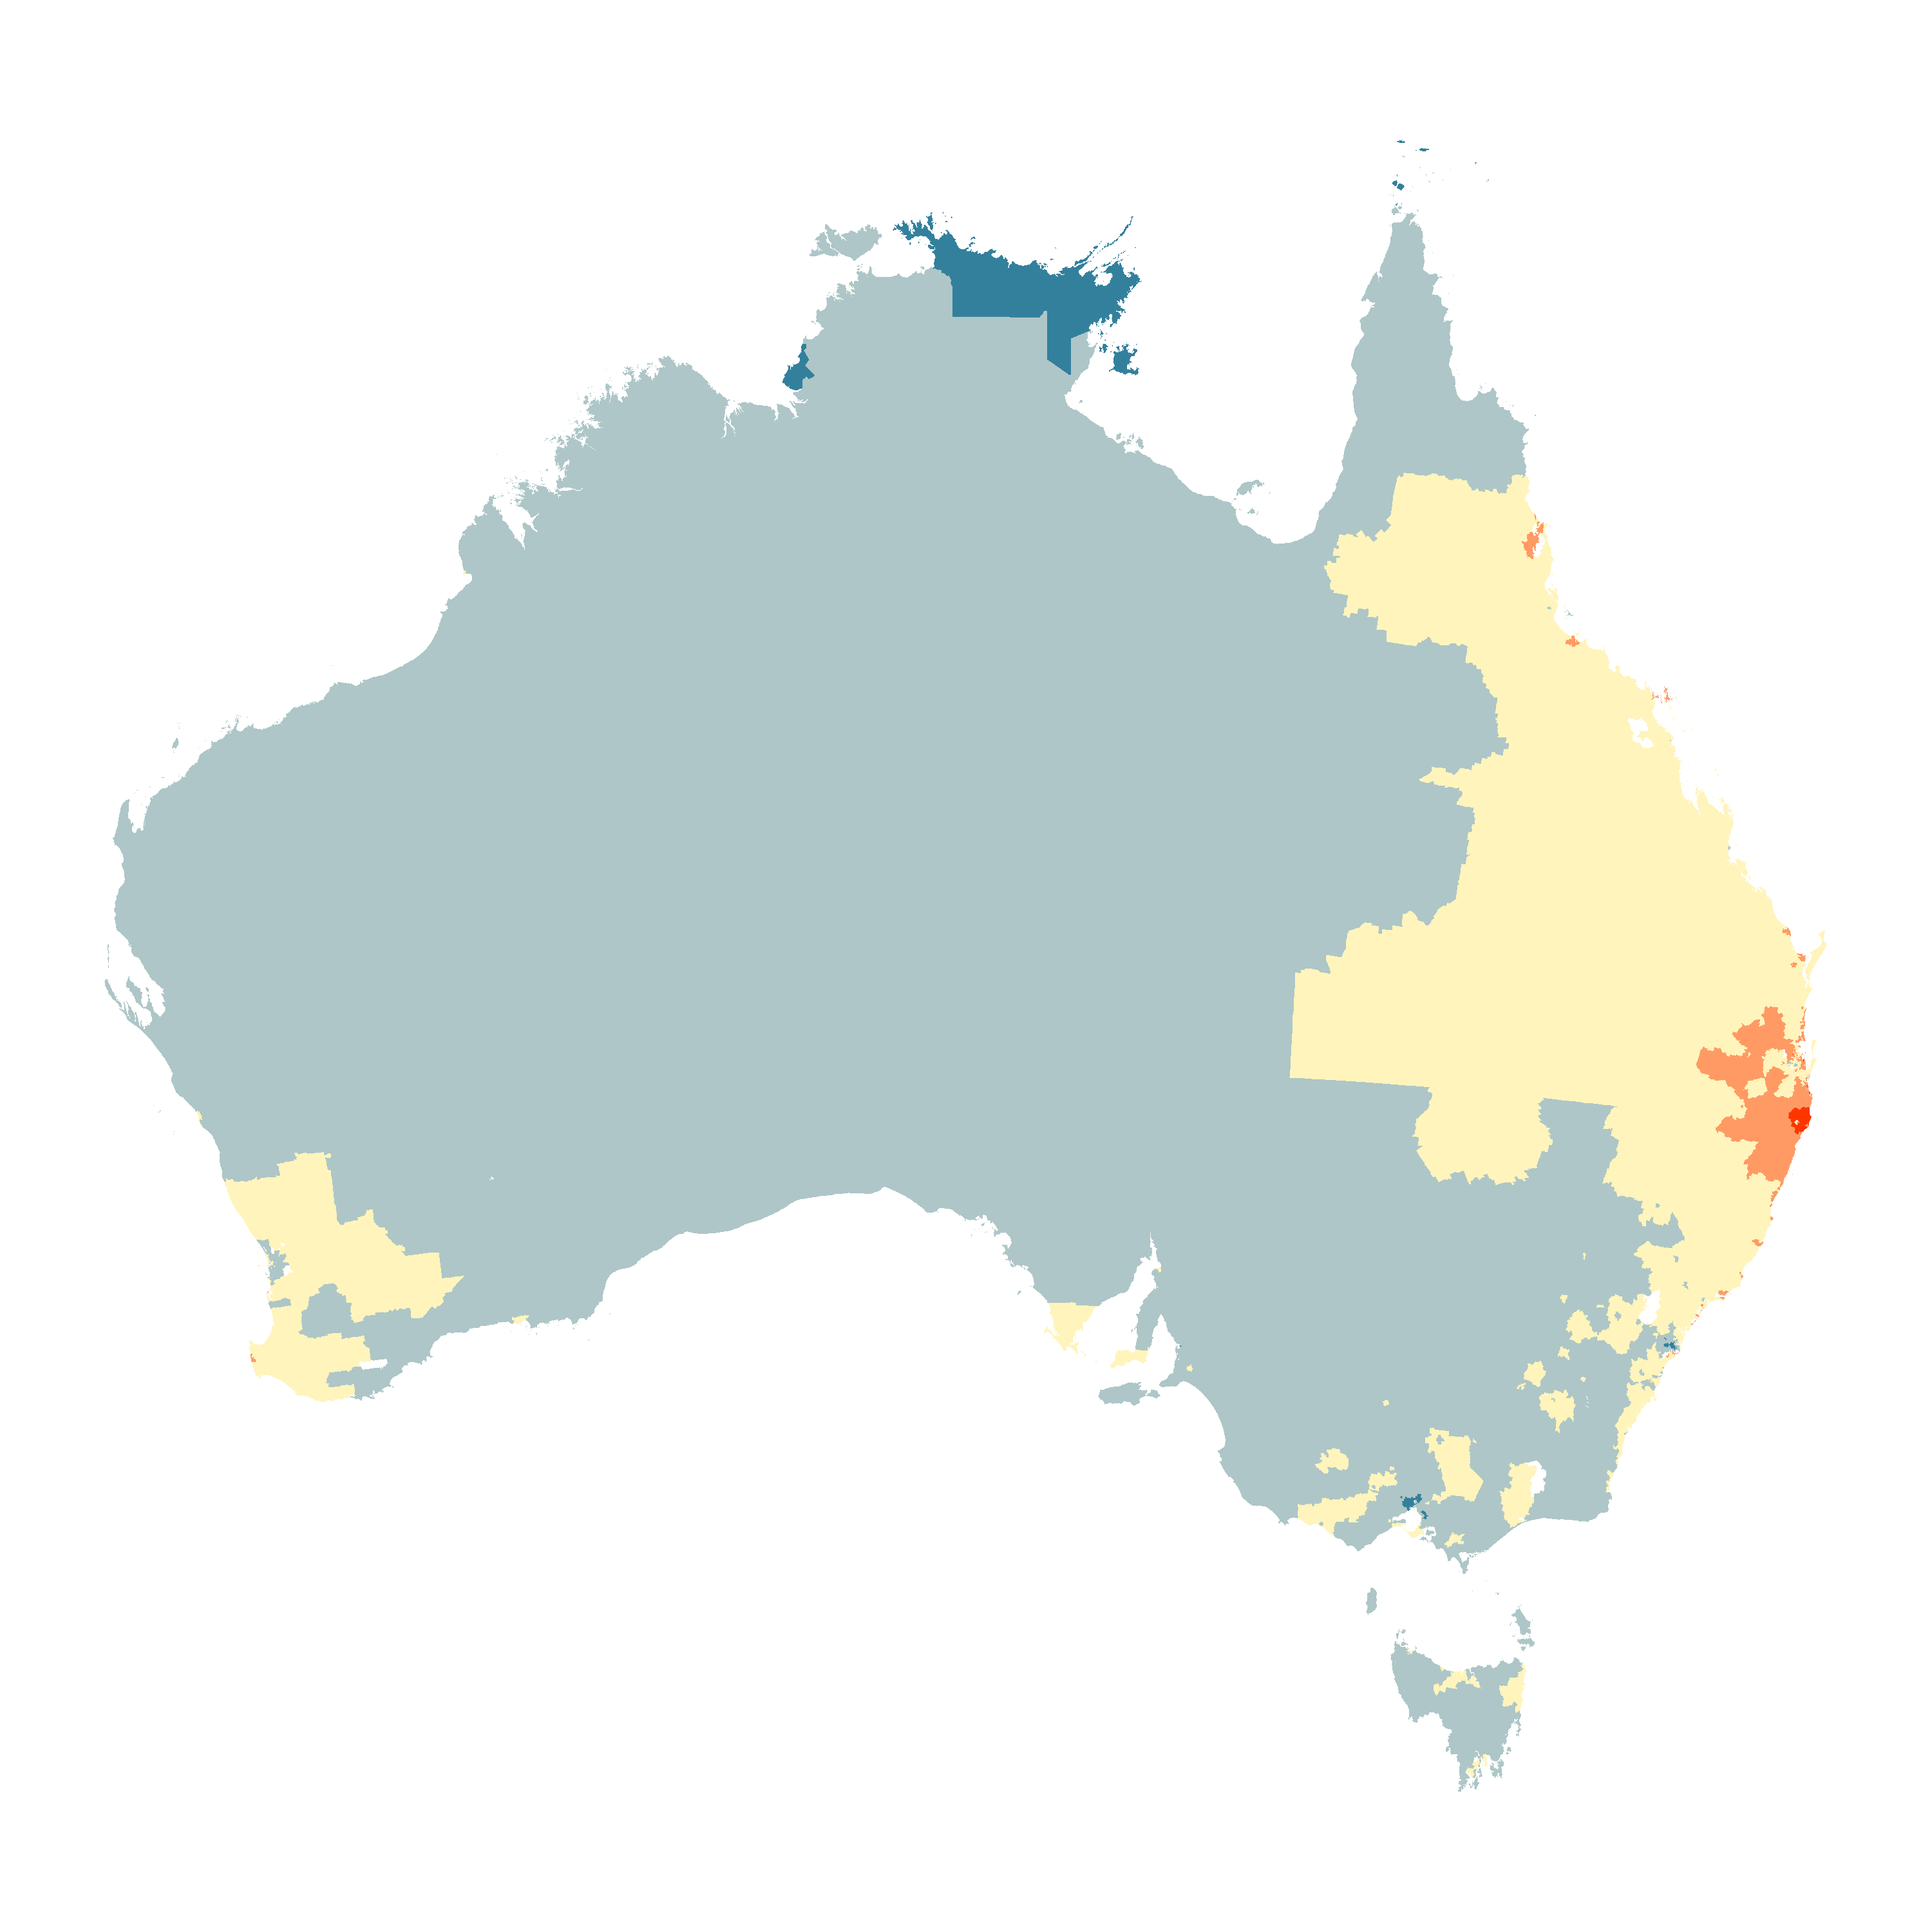
\includegraphics[width=14cm]{figs/aus_melanoma_p.png}
\caption{\label{fig:melanoma-geo}A choropleth map of the Statistical Areas of Australia at Level 2. The colours communicate the value of the estimated SIR of Melanoma for males, they range from much lower than average (blue) to much higher than average (red)}
\end{figure}

Alternative mapping methods allow increased understanding of the spatial
distribution of a variable across the population, by fairly representing
the population in each administrative area \citep{TAAM}. This
acknowledges that the number of residents can be different but
recognises that each area, or person within it is equally important.

This paper contains a discussion of Existing Mapping Practices in
Section 2. This is followed by details of the Algorithm in Section 3.
Section 4 describes the implementation of the algorithm in the
\texttt{sugarbag} package. Section 5 outlines the use and benefits of
animation.

\hypertarget{existing-mapping-practices}{%
\subsection{Existing Mapping
Practices}\label{existing-mapping-practices}}

There are several established alternative visualisation methods. Tile
maps, Rectangular cartograms \citep{ORC} and Dorling cartograms
\citep{ACTUC} all use one simple shape to represent each geographic
unit. They all minimise the emphasis on the size or shape of the
geographic areas. These alternative map displays focus on the
relationship between neighbours, attempting to preserve connections, and
disregard the unique shapes of the administrative boundaries. Figure
\ref{fig:nsw_grid} shows a collection of alternative map displays, this
includes a) a contiguous cartogram, b) a non-contiguous cartogram, c) a
Dorling cartogram and d) a hexagon tile map. Each Statistical Area at
Level 2 (SA2) \citep{abs2011} was designed to represent a community.
These administrative areas are often used to aggregate census data and
used to understand demographics of the Australian population.

The familiar choropleth map display is often used to allow the user to
orient themselves. However, the emphasis on the land mass diminishes the
features of the distribution in densely populated communities due to the
small size on the display \citep{ACTUC}. The unique shapes of boundaries
can be helpful for orienting users but may not contribute to their
understanding of the spatial disease distribution as many of the
communities are not visible in a choropleth display \citep{TVSSS}. This
presents an opportunity for explicit map transformations to improve
communication of distributions \citep{CBATCC}. In figure
\ref{fig:nsw_grid}a) the choropleth map is presented with the
alternative maps to allow for comparisons to be made.

\begin{Schunk}

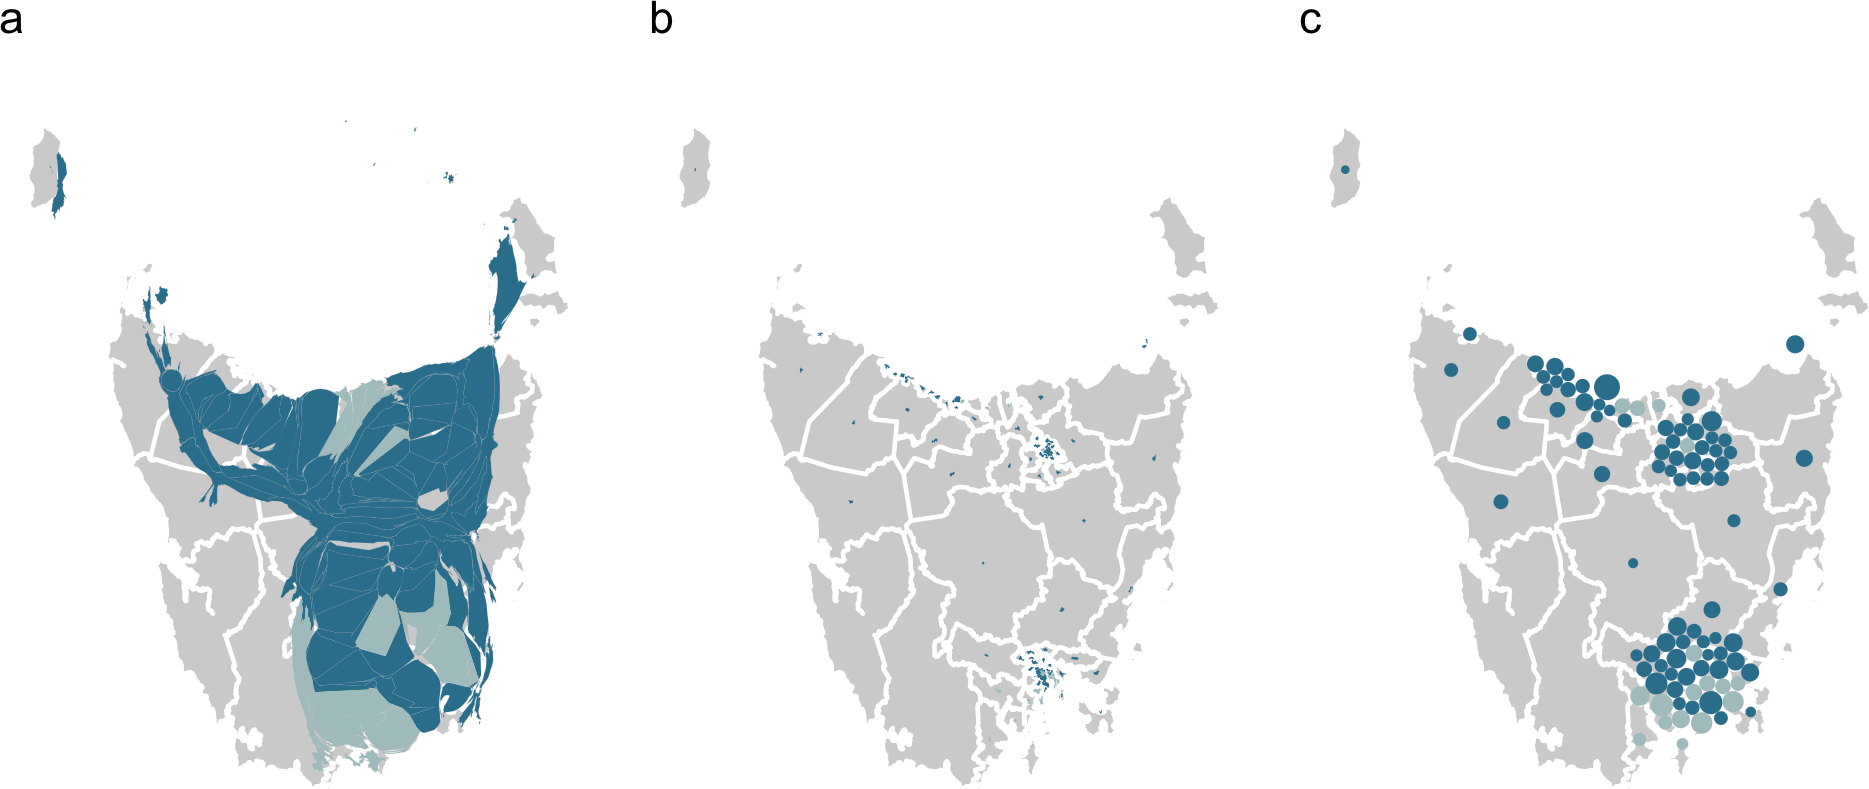
\includegraphics[width=0.9\linewidth]{kobakian-cook_files/figure-latex/tas_displays-1} \end{Schunk}

When communicating information that is relevant to the population, each
member of the population can be given equal representation by
transforming the map \citep{TVSSS}. The impact of a disease over
connected communities can be seen by allowing the boundaries to maintain
connection in the transformed display. The contiguous cartogram
displayed in figure \ref{fig:nsw_grid}b) draws attention to smaller
geographic units when they are rescaled according to the population
\citep{DMAHP}. These new shapes can now be coloured to represent a
second variable. This display can create twisted and unfamiliar shapes
from the geographic units as the algorithms must satisfy the topology
conditions, especially when there are communities located geographically
far from their neighbours \citep{TVSSS}. This shown in the northern SA2s
of Tasmania with an average (yellow) estimated SIR of Melanoma for
males.

The non-contiguous cartogram in figure \ref{fig:nsw_grid}c) also uses
the population to rescale the geographic units. Unlike the contiguous
cartogram, the SA2 areas maintain their geographic shape, but they may
not retain the connection with their neighbours. The population of the
SA2 areas is used to scale the geographic units in the non-contiguous
cartogram \citep{NAC}. The amount of white space can be meaningful in
non-contiguous cartograms \citep{ECGC}, in this example the disparity
between large rural areas and small urban areas means that the city of
Hobart, shown in the inset map looks reasonable, but these units are not
visible in the context of the Tasmania state map. Depending on the
difference between the population and geographic land size, the amount
of white space can also prevent meaningful understanding of the
distribution \citep{TVSSS}.

The Dorling cartogram presents each geographic unit as a circle, the
size of the circle is scaled according to the population value of each
area \citep{ACTUC}. Figure \ref{fig:nsw_grid}d) shows the Tasmania SA2
areas as an individual circle located as close as possible to the
geographic centroid location. This map draws attention to the collection
of coastal cities in Tasmania that were not apparent in figure
\ref{fig:nsw_grid} a), b) or c).

\hypertarget{algorithm}{%
\subsection{Algorithm}\label{algorithm}}

The purpose of this algorithm is to create a map display that highlights
the spatial distributions for populations. There has been an increasing
need for displays that recognise the large number of people that live in
dense urban environments. The algorithm intends to maintain the spatial
relationships of a group of geographic units in two ways: between each
unit and its neighbours; and between each unit and the closest focal
point. The algorithm allocates geographic units to a representative
hexagon, in order of their proximity to the closest focal point.

The algorithm is named for the \emph{Trigona carbonaria} bee species.
Native to northern and eastern Australia this stingless species builds
flat layers of hexagonal brood cells, spiralling out from a central
point \citep{PH}. This hive design inspired the use of multiple focal
points in the algorithm, individual spirals are constructed outward from
various points on the geographic map base.

There are three key steps performed to create a tessellated hexagon tile
map. First derive the set of centroids from the polygons provided, then
create the grid of hexagons locations. These two steps are defined in
the blue left column of the flow chart in Figure
\ref{fig:sugarbag_flow}. Each centroid can then be allocated to an
available hexagon location. The steps for the allocation process are
detailed in the right column of Figure \ref{fig:sugarbag_flow}. To make
tessellated plots, the point locations are converted to hexagon shapes,
with the hexagon size used in the grid.

\begin{figure}
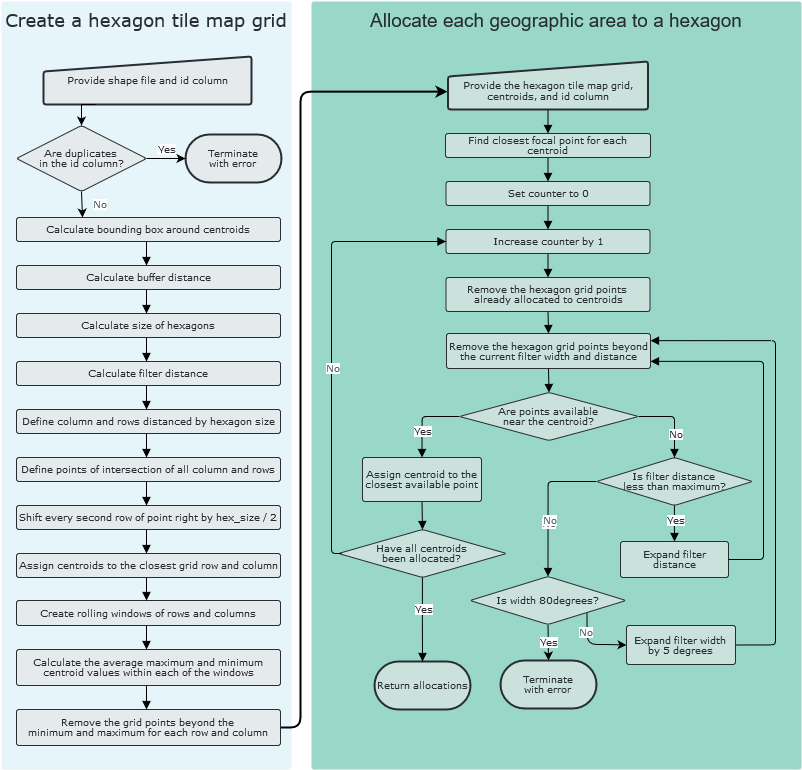
\includegraphics[width=14cm]{figs/sugarbag flow.png}
\caption{\label{fig:sugarbag_flow}A flow diagram detailing the necessary steps to create a hexagon tile map.}
\end{figure}

\hypertarget{user-choices}{%
\paragraph{User choices}\label{user-choices}}

Only two inputs are necessary to begin using the algorithm, the shape
file, and the id variable. The id column should uniquely identify each
geographic unit in the shape file.

The centroids can be derived from the shape file. The amount of
centroids is used to determine a hexagon size. The derived centroids are
a necessary input for an appropriate grid to be constructed, in which
each grid point is located a hexagon size distance from the next closest
point in all six directions. The grid will initially cover the entire
map space, encompassing all the centroid locations and will extend in
all directions to the extent of the buffer distance. This buffer
distance can be helpful to account for densely populated coastal areas,
allowing the use of the sea for hexagon locations. The hexagon size will
likely need adjustments depending on the density of the population.

The centroids derived from the shape file are necessary inputs when
creating a grid. The creation of the grid and filtering out the points
unlikely to be used in the hexagon map results in the hexagon tile map
grid. At this point, the centroid set and the grid become the necessary
inputs to the allocation process.

A set of reference locations can be provided as focal points, such as
capital cities of states or countries. Using focal points, the algorithm
will create the order of allocation in order of the closest centroid
locations to the focal points. Alternatively, a user can specify the
variable that should be used to determine the order for the allocation.
When allocating representative hexagons, the width parameter can be used
to determine the flexibility of positioning using the relationship with
the nearest reference location. A larger width parameter will increase
the amount of available hexagon locations nearer to the centroid of the
geographic location. A smaller width will maintain the orientation from
the focal point to the centroid when selecting the hexagon location,
however this could mean it is placed further from the centre of the
cluster.

\hypertarget{implementation}{%
\subsection{Implementation}\label{implementation}}

Hexagon tile maps can be useful to understand a distribution across a
collection of geographic areas. However, these maps are not easily
drawn, especially as the number of areas increases. This algorithm was
created to automate this process, and reduce the manual load involved in
creating and implementing alternative displays. This allows map makers
and data communicators to allocate their time to choosing the most
effective display, rather than manually creating them.

The \texttt{sugarbag} package has been written for R software, it
contains a set of functions that help R users to create a hexagon tile
map. The algorithm presented in the \texttt{sugarbag} package operates
on a set of simple feature geometry objects \citep{sf}, this package
allows R users to create \texttt{sf} objects by importing polygons
stored in various formats. Users should provide a set of polygons that
define geographic units by their administrative boundaries. The
functions arrange the geographic units in order of proximity to a set of
locations provided, such as the centre of capital cities. The centroid
location of each geographic unit is used to measure the proximity. It
emphasises the capital cities as population hubs, rather than
emphasizing the size of large, rural geographic units.

A user can tweak the parameters of the hexagon map using the additional
arguments to the \texttt{create\_hexmap} function, these options may
affect the speed of the creation.

\hypertarget{creating-a-hexagon-tile-map}{%
\paragraph{Creating a hexagon tile
map}\label{creating-a-hexagon-tile-map}}

The following code creates the hexagon tile map for all the Statistical
Areas at Level 2 in Tasmania. These steps can be executed by the main
function, \texttt{create\_hexmap}, or can be implemented separately for
more flexibility.

If a user would like to perform each of the steps of the algorithm
themselves, the necessary inputs will change for each function.

Users may choose to only use the \texttt{allocate} function when they
wish to use a set of centroids, rather than \citep{sf} polygons.

\hypertarget{polygon-set}{%
\paragraph{Polygon set}\label{polygon-set}}

The polygon set of Statistical Areas at Level 2 (SA2) \citep{abs2011} of
Tasmania in 2011 is provided with the \texttt{sugarbag} package as
\texttt{tas\_sa2}. A single column of the data set is used to identify
the unique areas. In this case, the unique SA2 names for each SA2 have
been used.

The longitude and latitude centre of the capital cities of Australia are
used as focal points to allocate each geographic area around the closest
capital city. Hobart will be the common focal point, as this example
uses only the areas in the state of Tasmania.

The buffer distance, hexagon size, hexagon amount to filter and width of
angle are parameters that will be determined within
\texttt{create\_hexmap} if they are not provided. They are created as
they are needed throughout the following example.

\hypertarget{step-1-derive-the-set-of-centroid-points}{%
\paragraph{Step 1: Derive the set of centroid
points}\label{step-1-derive-the-set-of-centroid-points}}

A set of centroids may be used directly. The set of polygons should be
provided as an \texttt{sf} object, this is a data frame containing a
\texttt{geometry} column. The \texttt{read\_shape} function can assist
in creating this object for use in \texttt{R}.

The centroids can be derived from the set of polygons using the
\texttt{create\_centroids} function:

\begin{figure}[h]
\centering
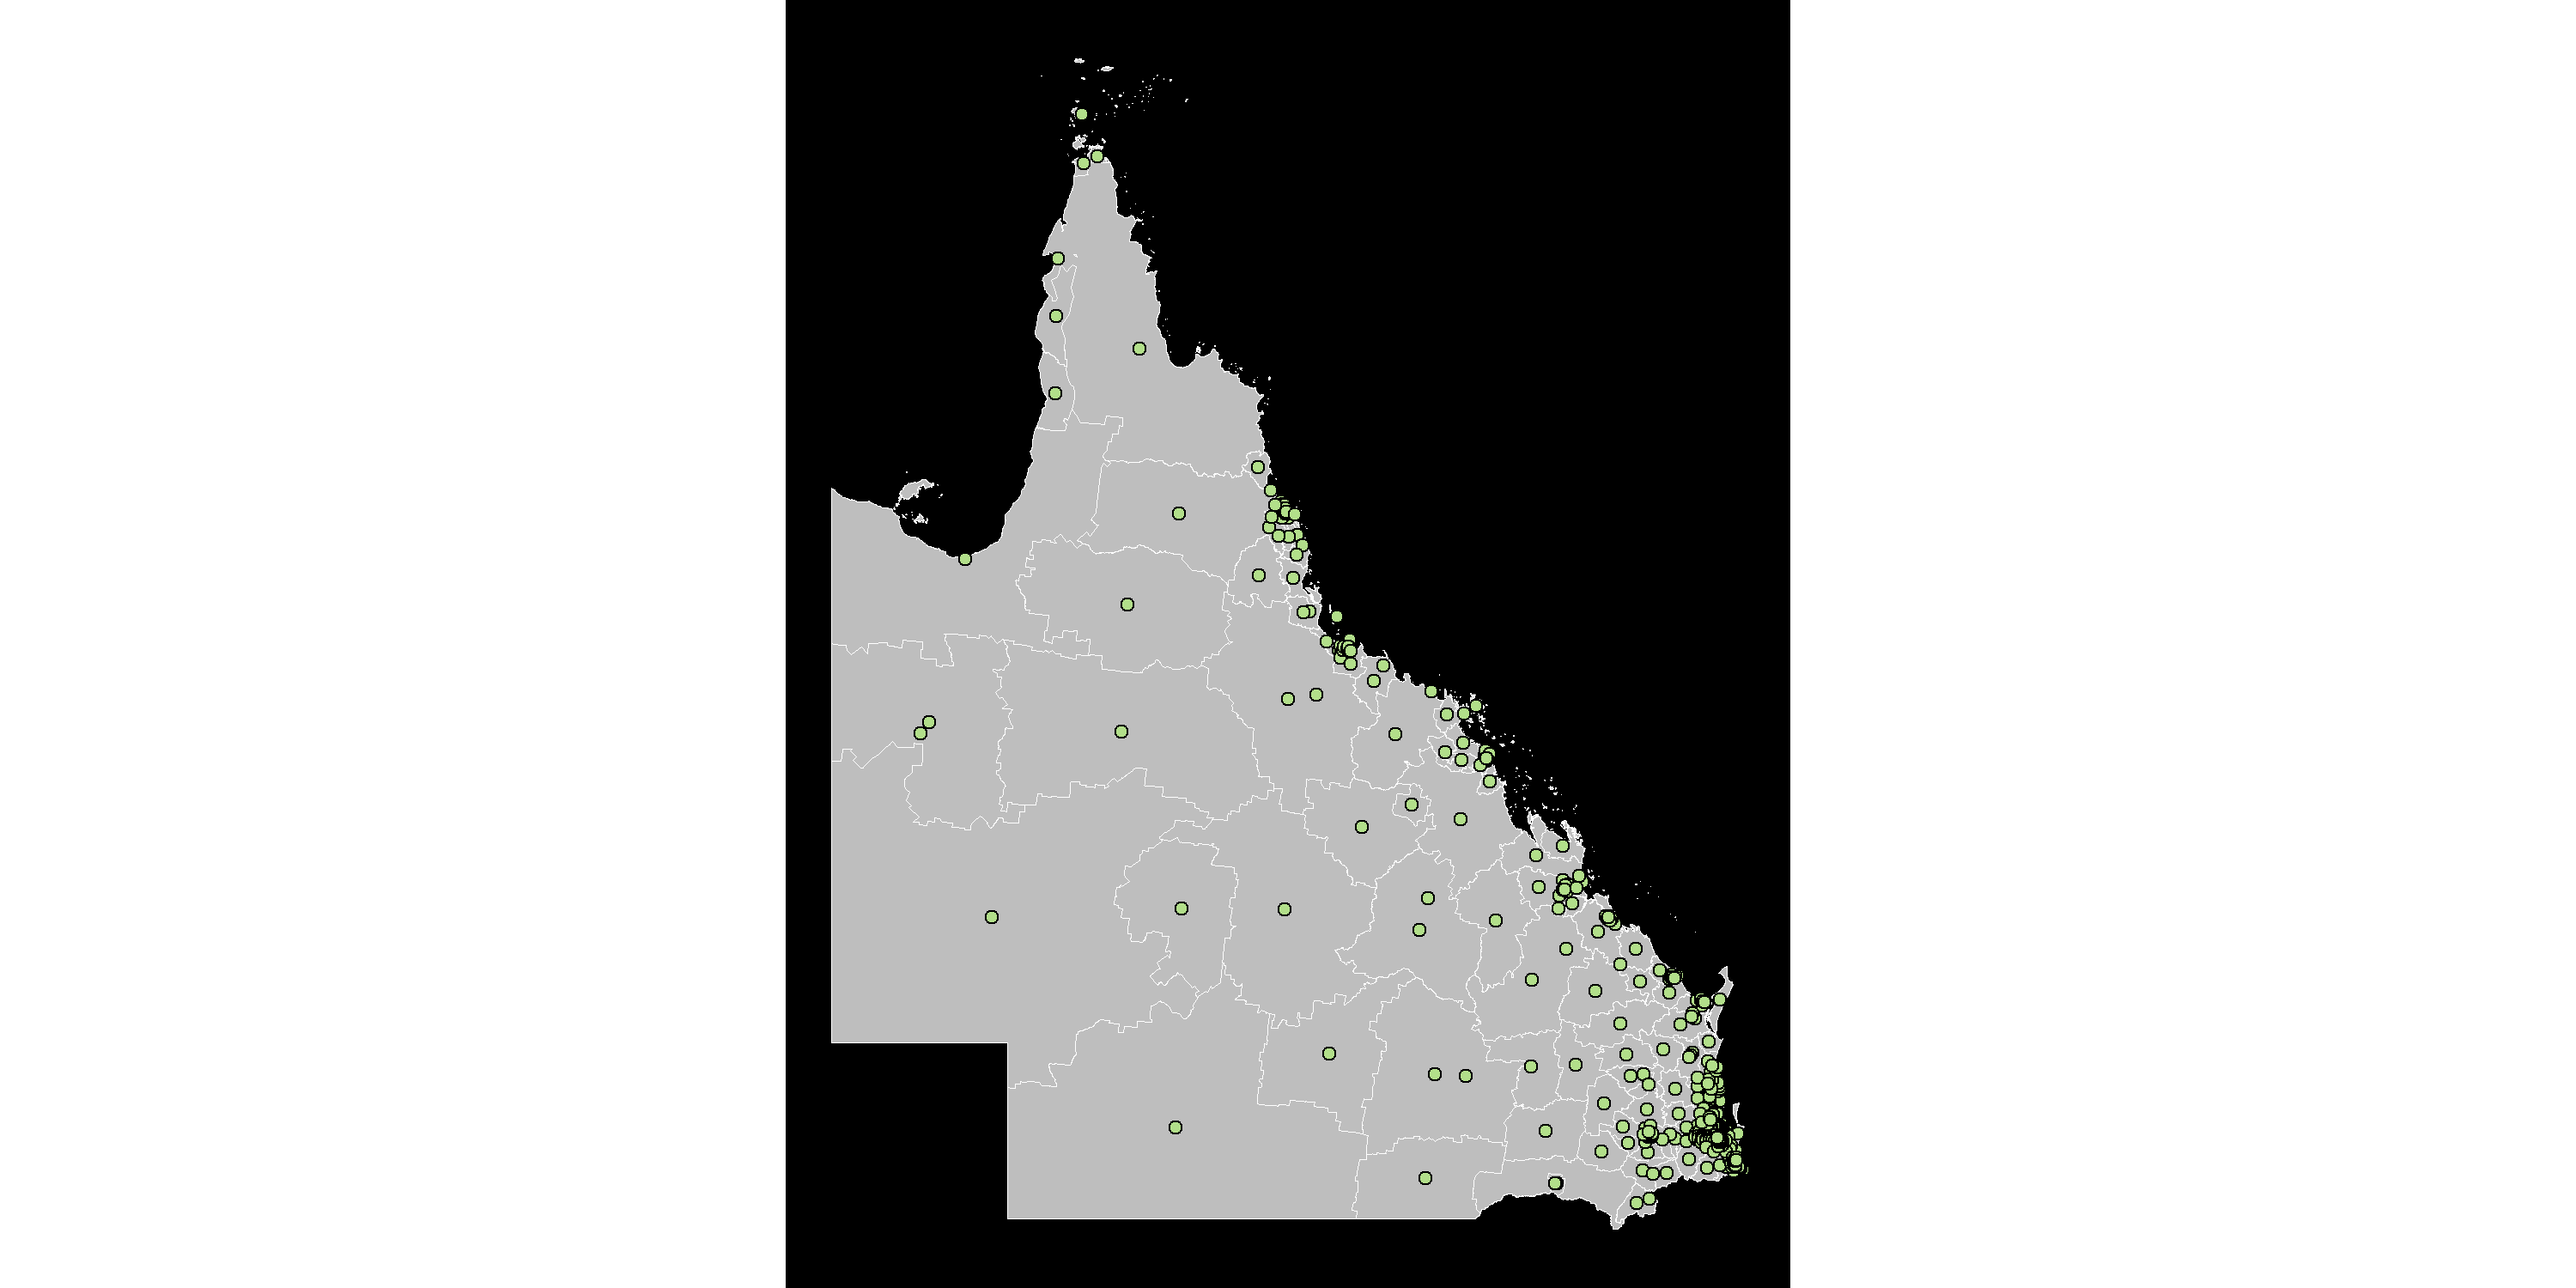
\includegraphics[width=14cm]{figs/1centroids.png}
\caption{\label{fig:centroids_plot}The geographic shapes of the Statistical Areas of Tasmania at Level 2. The points show the locations of the centroids of the SA2 areas.}
\end{figure}

\hypertarget{step-2-create-the-hexagon-grid-points}{%
\paragraph{Step 2: Create the hexagon grid
points}\label{step-2-create-the-hexagon-grid-points}}

A grid is created to ensure tessellation between the hexagons that
represent the geographic units on a hexagon tile map.

The grid of possible hexagon locations is made using the
\texttt{create\_grid} function. It uses the centroids, the hexagon size
and the buffer distance.

\hypertarget{creating-a-tessellated-grid}{%
\subparagraph{Creating a tessellated
grid}\label{creating-a-tessellated-grid}}

A set of longitude columns, and latitude rows are created to define the
locations of the hexagons. The distance between each row and column is
the size specified by \texttt{hex\_size}. Equally spaced columns are
created from the minimum longitude minus the buffer distance, up to the
maximum longitude plus the buffer distance. Similarly, the rows are
created from the latitude values and the buffer distance. A unique
hexagon location is created from all intersections of the longitude
columns and latitude rows. Figure \ref{fig:grid2} shows the original
grid on the left, to allow for tessellating hexagons, every second
latitude row on the grid is shifted right, by half of the hexagon size.
The grid for tessellation is shown on the right.

\begin{figure}[h]
\centering
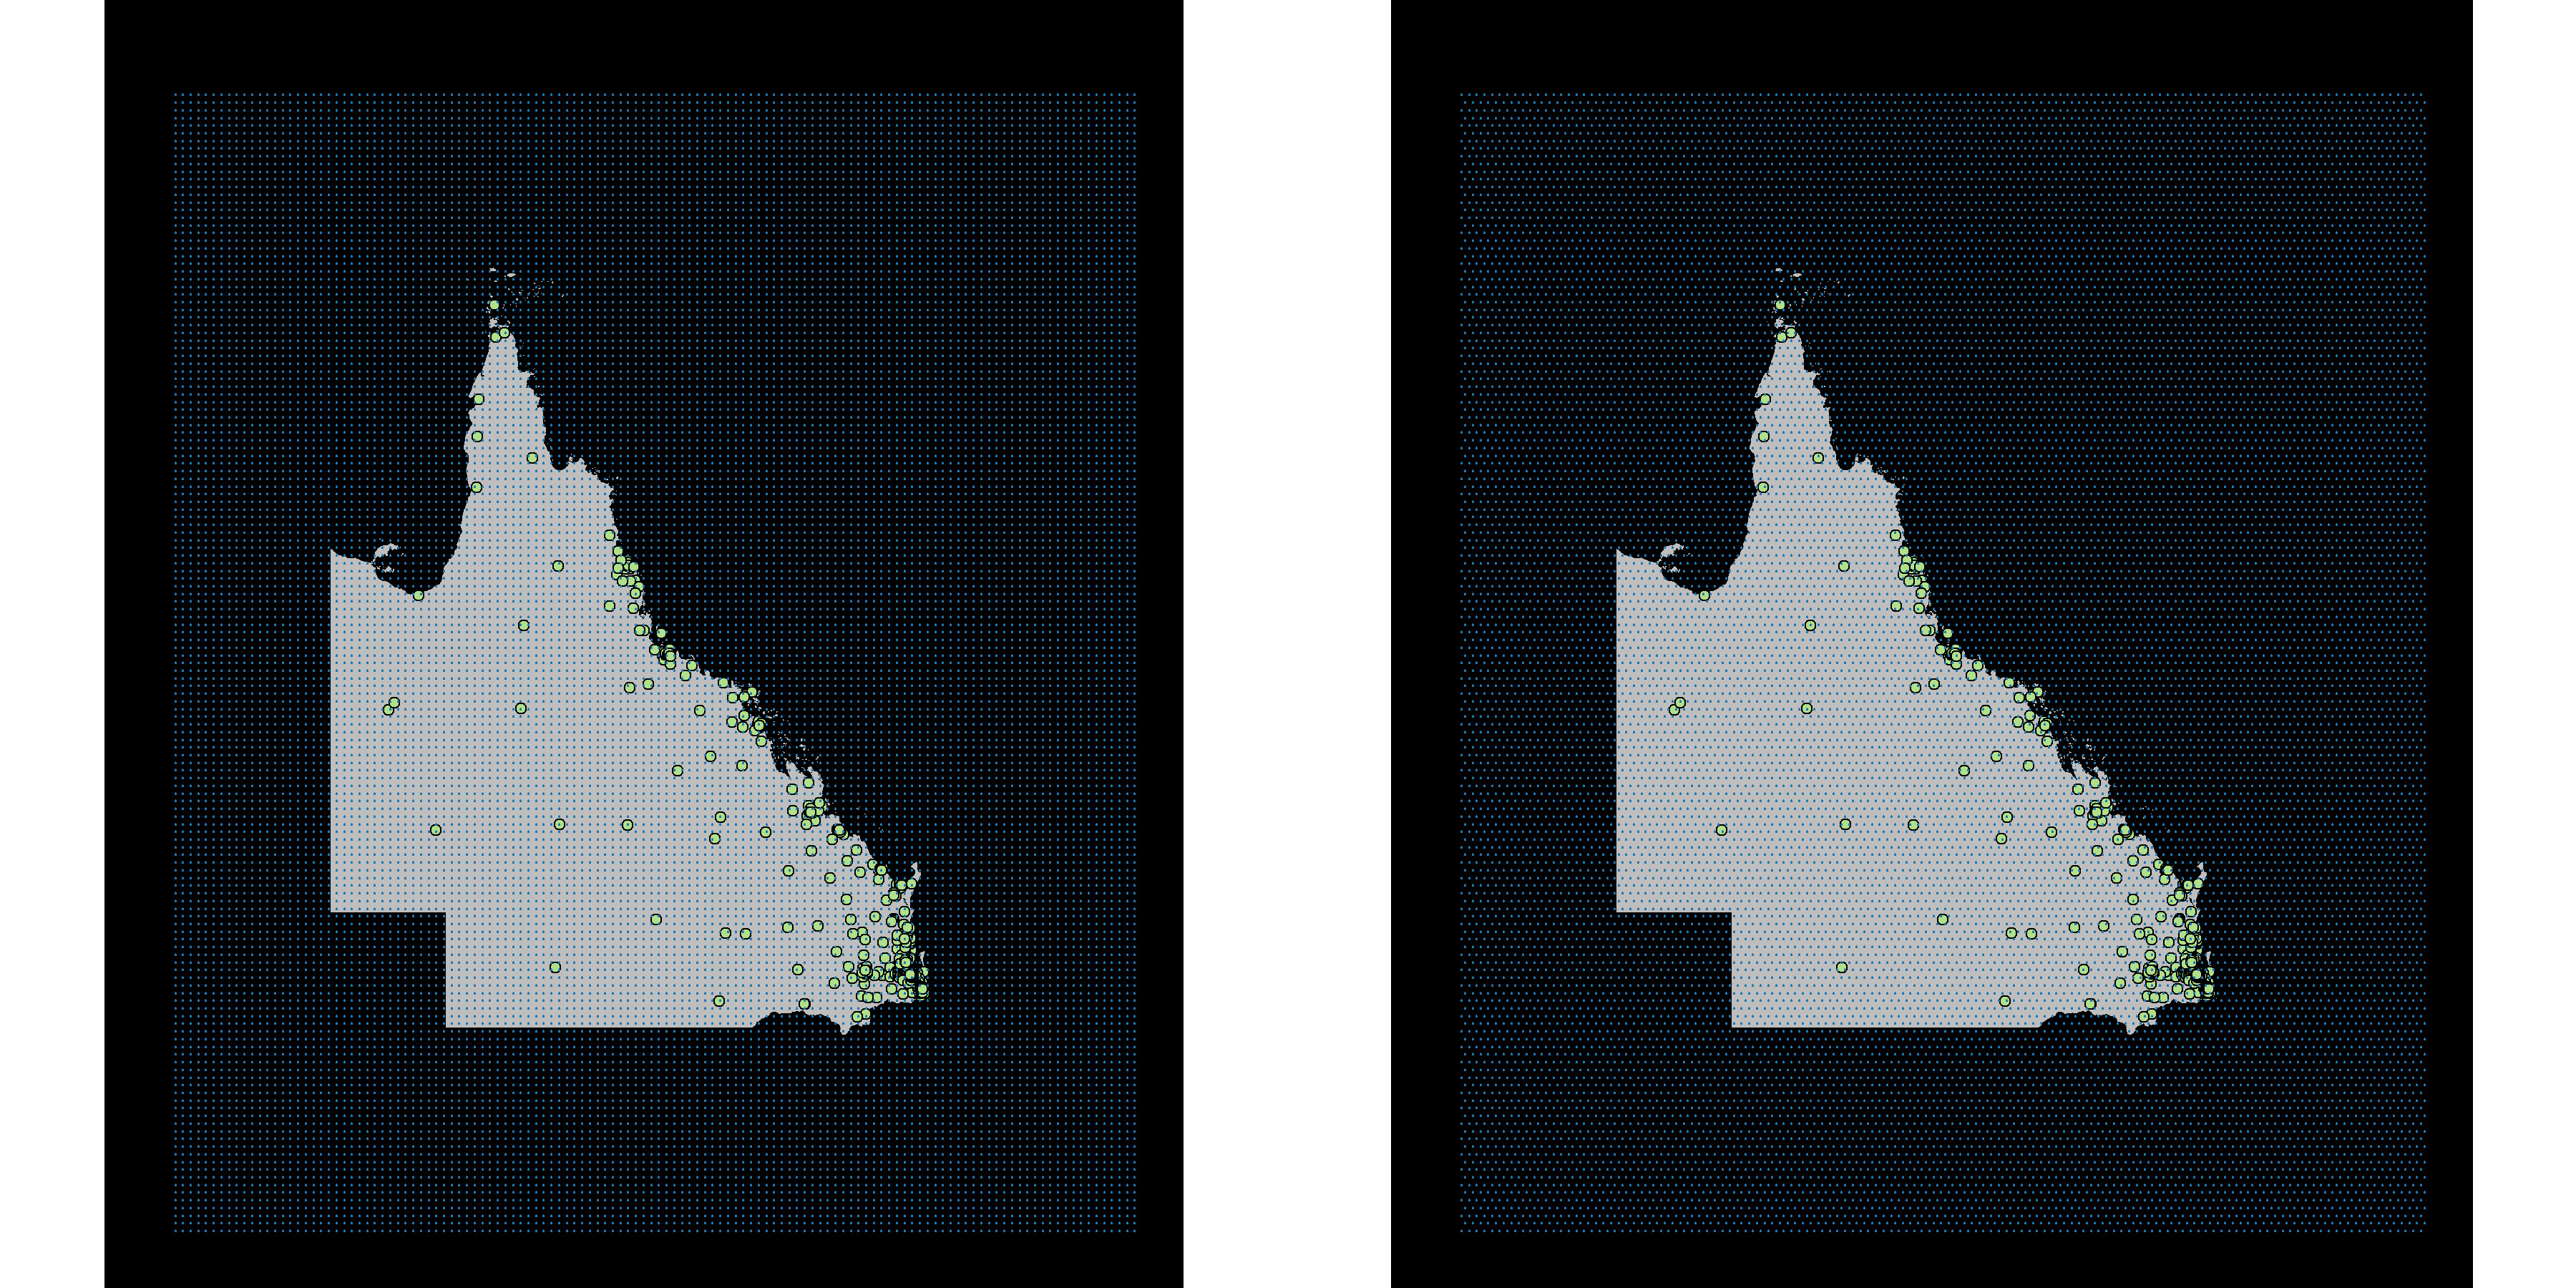
\includegraphics[width=16cm]{figs/2grid.png}
\caption{\label{fig:grid2}Grid points to create a hexagon tile map.}
\end{figure}

\hypertarget{rolling-windows}{%
\subparagraph{Rolling windows}\label{rolling-windows}}

Not all of the grid points will be used, especially if islands result in
a large grid space. To filter the grid for appropriate hexagon locations
for allocation, the \texttt{create\_buffer} function is used by
\texttt{create\_grid}. It finds the grid points needed to best capture
the set of centroids on a hexagon tile map.

The closest latitude row and longitude column are found for each
centroid location. Then rows and columns of centroids are divided into
20 groups. The amount of rows in each latitude group and the amount of
columns in each longitude group are used as the width of rolling
windows. The rolling windows can be seen on the bottom and right of the
grid shown in Figure \ref{fig:filter-grid}. This will tailor the
available grid points to those most likely to be used. It also helps
reduce the amount of time taken, as it decreases the amount of points
considered for each centroid allocation.

The first rolling window function finds the minimum and maximum centroid
values for the sliding window groups of longitude columns and the groups
of latitude rows.

The second rolling window function finds the average of the rolling
minimum and maximum centroid values, for the longitude columns and
latitude rows.

\hypertarget{filtering-the-grid}{%
\subparagraph{Filtering the grid}\label{filtering-the-grid}}

The grid points are kept only if they fall between the rolling average
of the minimum and maximum centroid values after accounting for the
buffer distance, for each row and column of the grid. The sparsely
populated South-West region of National Park has much fewer points
available compared to the South-East region containing the city of
Hobart.

\begin{figure}[h]
\centering
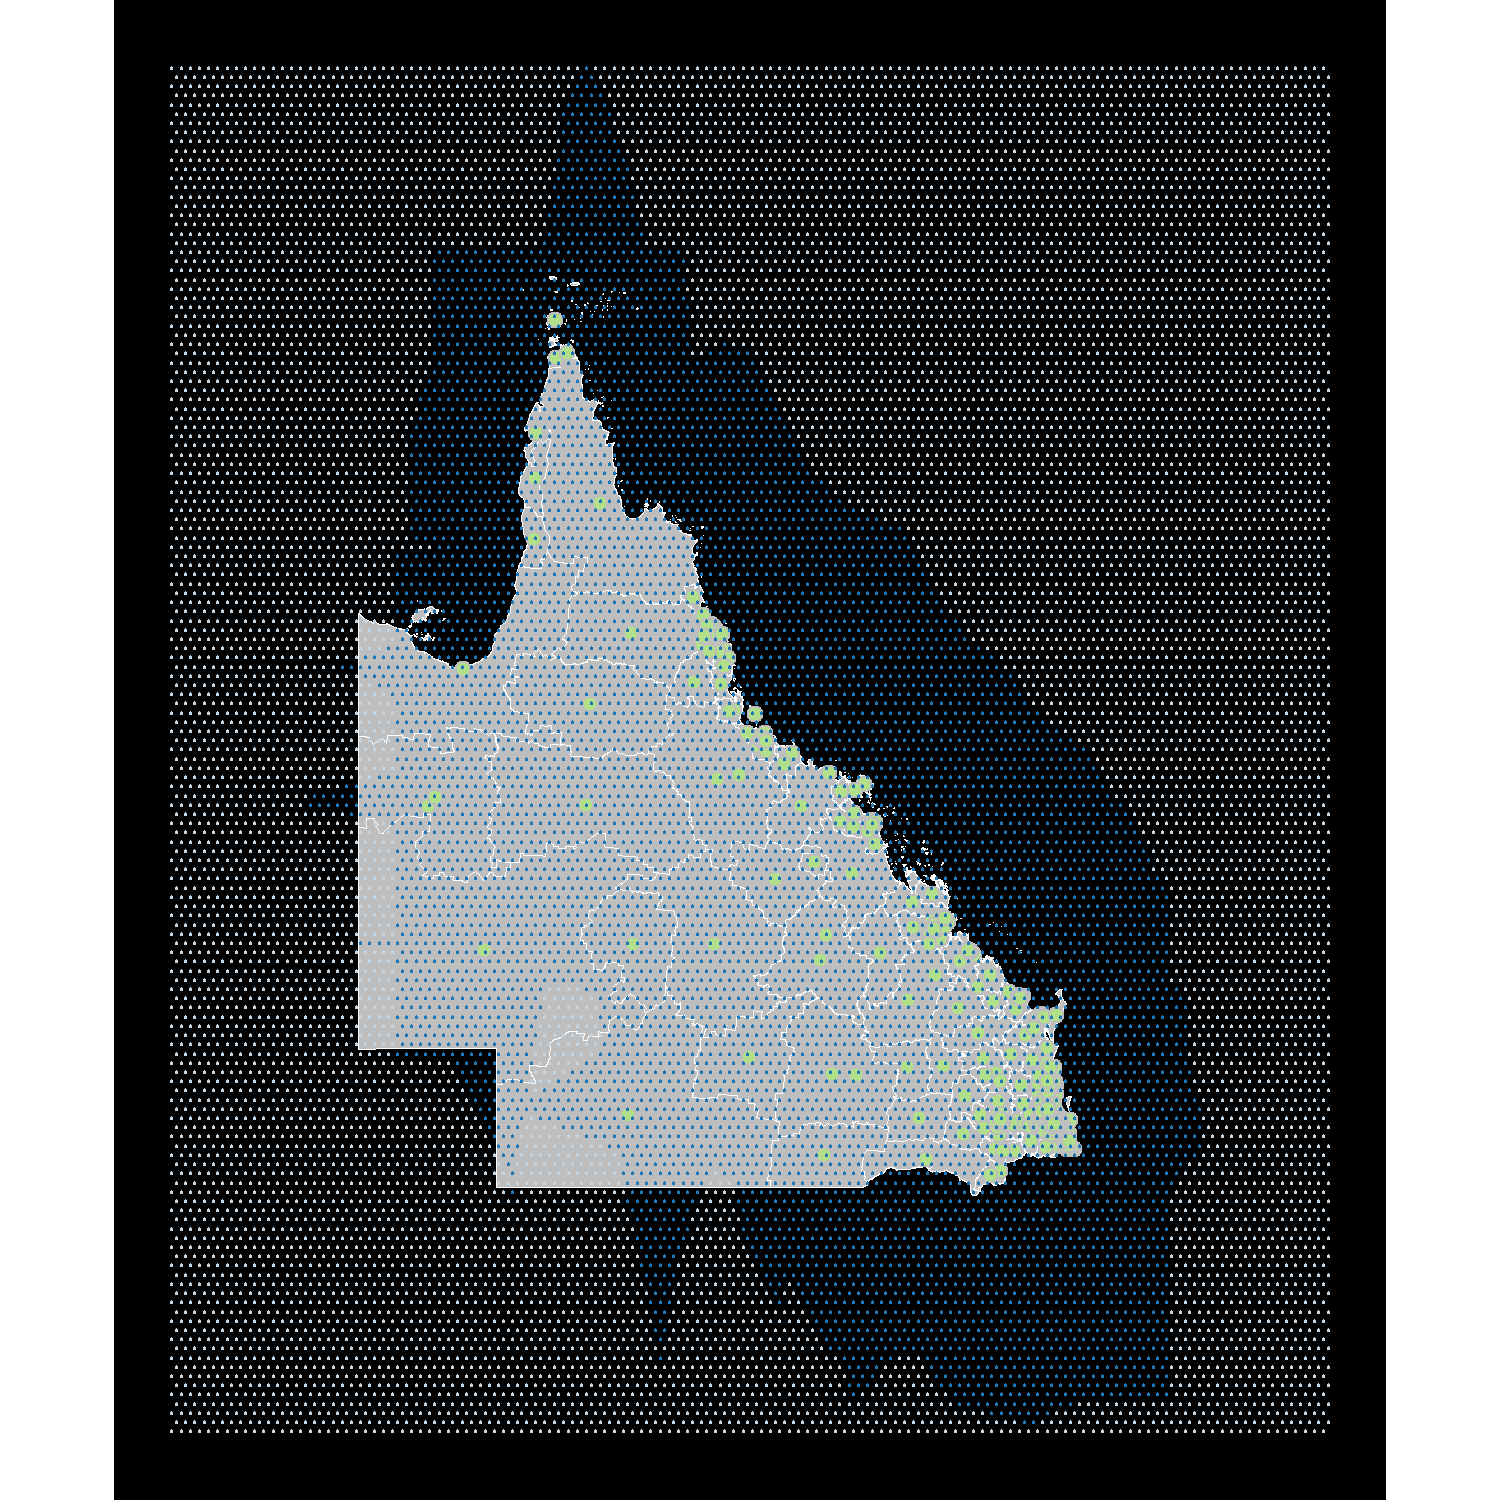
\includegraphics[width=10cm]{figs/3grid.png}
\caption{\label{fig:filter-grid}The remaining hexagon locations from all the possible points in the initial grid after the buffer is applied. The blue dots show the grid points left to choose from after the buffer step.}
\end{figure}

\hypertarget{centroid-to-focal-point-distance}{%
\subparagraph{Centroid to focal point
distance}\label{centroid-to-focal-point-distance}}

The distance between each centroid in the set, and each of the focal
points provided is calculated. The name of the closest focal point, and
the distance and angle from focal point to polygon centroid is joined to
polygon data set. To minimise time taken for this step only one option
is provided, Tasmania's capital city Hobart. The order for allocation is
determined by the distance between the polygon centroid and it's closest
focal point. The points are arranged from the centroid closest to the
focal point(s), to the furthest.

\hypertarget{step-3-allocate-each-centroid-to-a-hexagon-grid-point}{%
\paragraph{Step 3: Allocate each centroid to a hexagon grid
point}\label{step-3-allocate-each-centroid-to-a-hexagon-grid-point}}

Allocation of all centroids takes place using the set of polygon
centroids and the hexagon map grid. Centroid allocation begins with the
closest centroid to a focal point. This will preserve spatial
relationships with the focal point, as the inner city areas are
allocated first, they will be placed closest to the capital, and the
areas that are further will then be accommodated. The possible hexagon
grid points reduces by one after each allocation, then only those that
have not yet been allocated are considered.

The possible hexagon locations to consider for a centroid are determined
by the \texttt{hex\_filter}. This is the maximum amount of hexagons
between the centroid and the furthest considered hexagon. It is used to
subset possible grid points to only those surrounding the polygon
centroid within an appropriate range. A smaller distance will increase
speed, but can decrease accuracy when width of the angle increases.

The following example considers the first of the Statistical Areas at
Level 2. Within the algorithm, these steps are repeated for each
polygon.

\hypertarget{filter-the-grid-for-unassigned-hexagon-points}{%
\subparagraph{Filter the grid for unassigned hexagon
points}\label{filter-the-grid-for-unassigned-hexagon-points}}

Keeping only the available hexagon points prevents multiple geographic
units from being allocated to the same hexagon.

\hypertarget{filter-the-grid-points-for-those-closest-to-the-centroid}{%
\subparagraph{Filter the grid points for those closest to the
centroid}\label{filter-the-grid-points-for-those-closest-to-the-centroid}}

A box of possible hexagon locations around the centroid allows only the
closest points that are not yet assigned to be considered. The corners
of the box may not appear square if the buffer step has already removed
unnecessary points from over the ocean.

The algorithm then removes the outer corners of the square, creating a
circle of points, by only keeping points within a certain radial
distance around the original centroid location.

\begin{figure}[h]
\centering
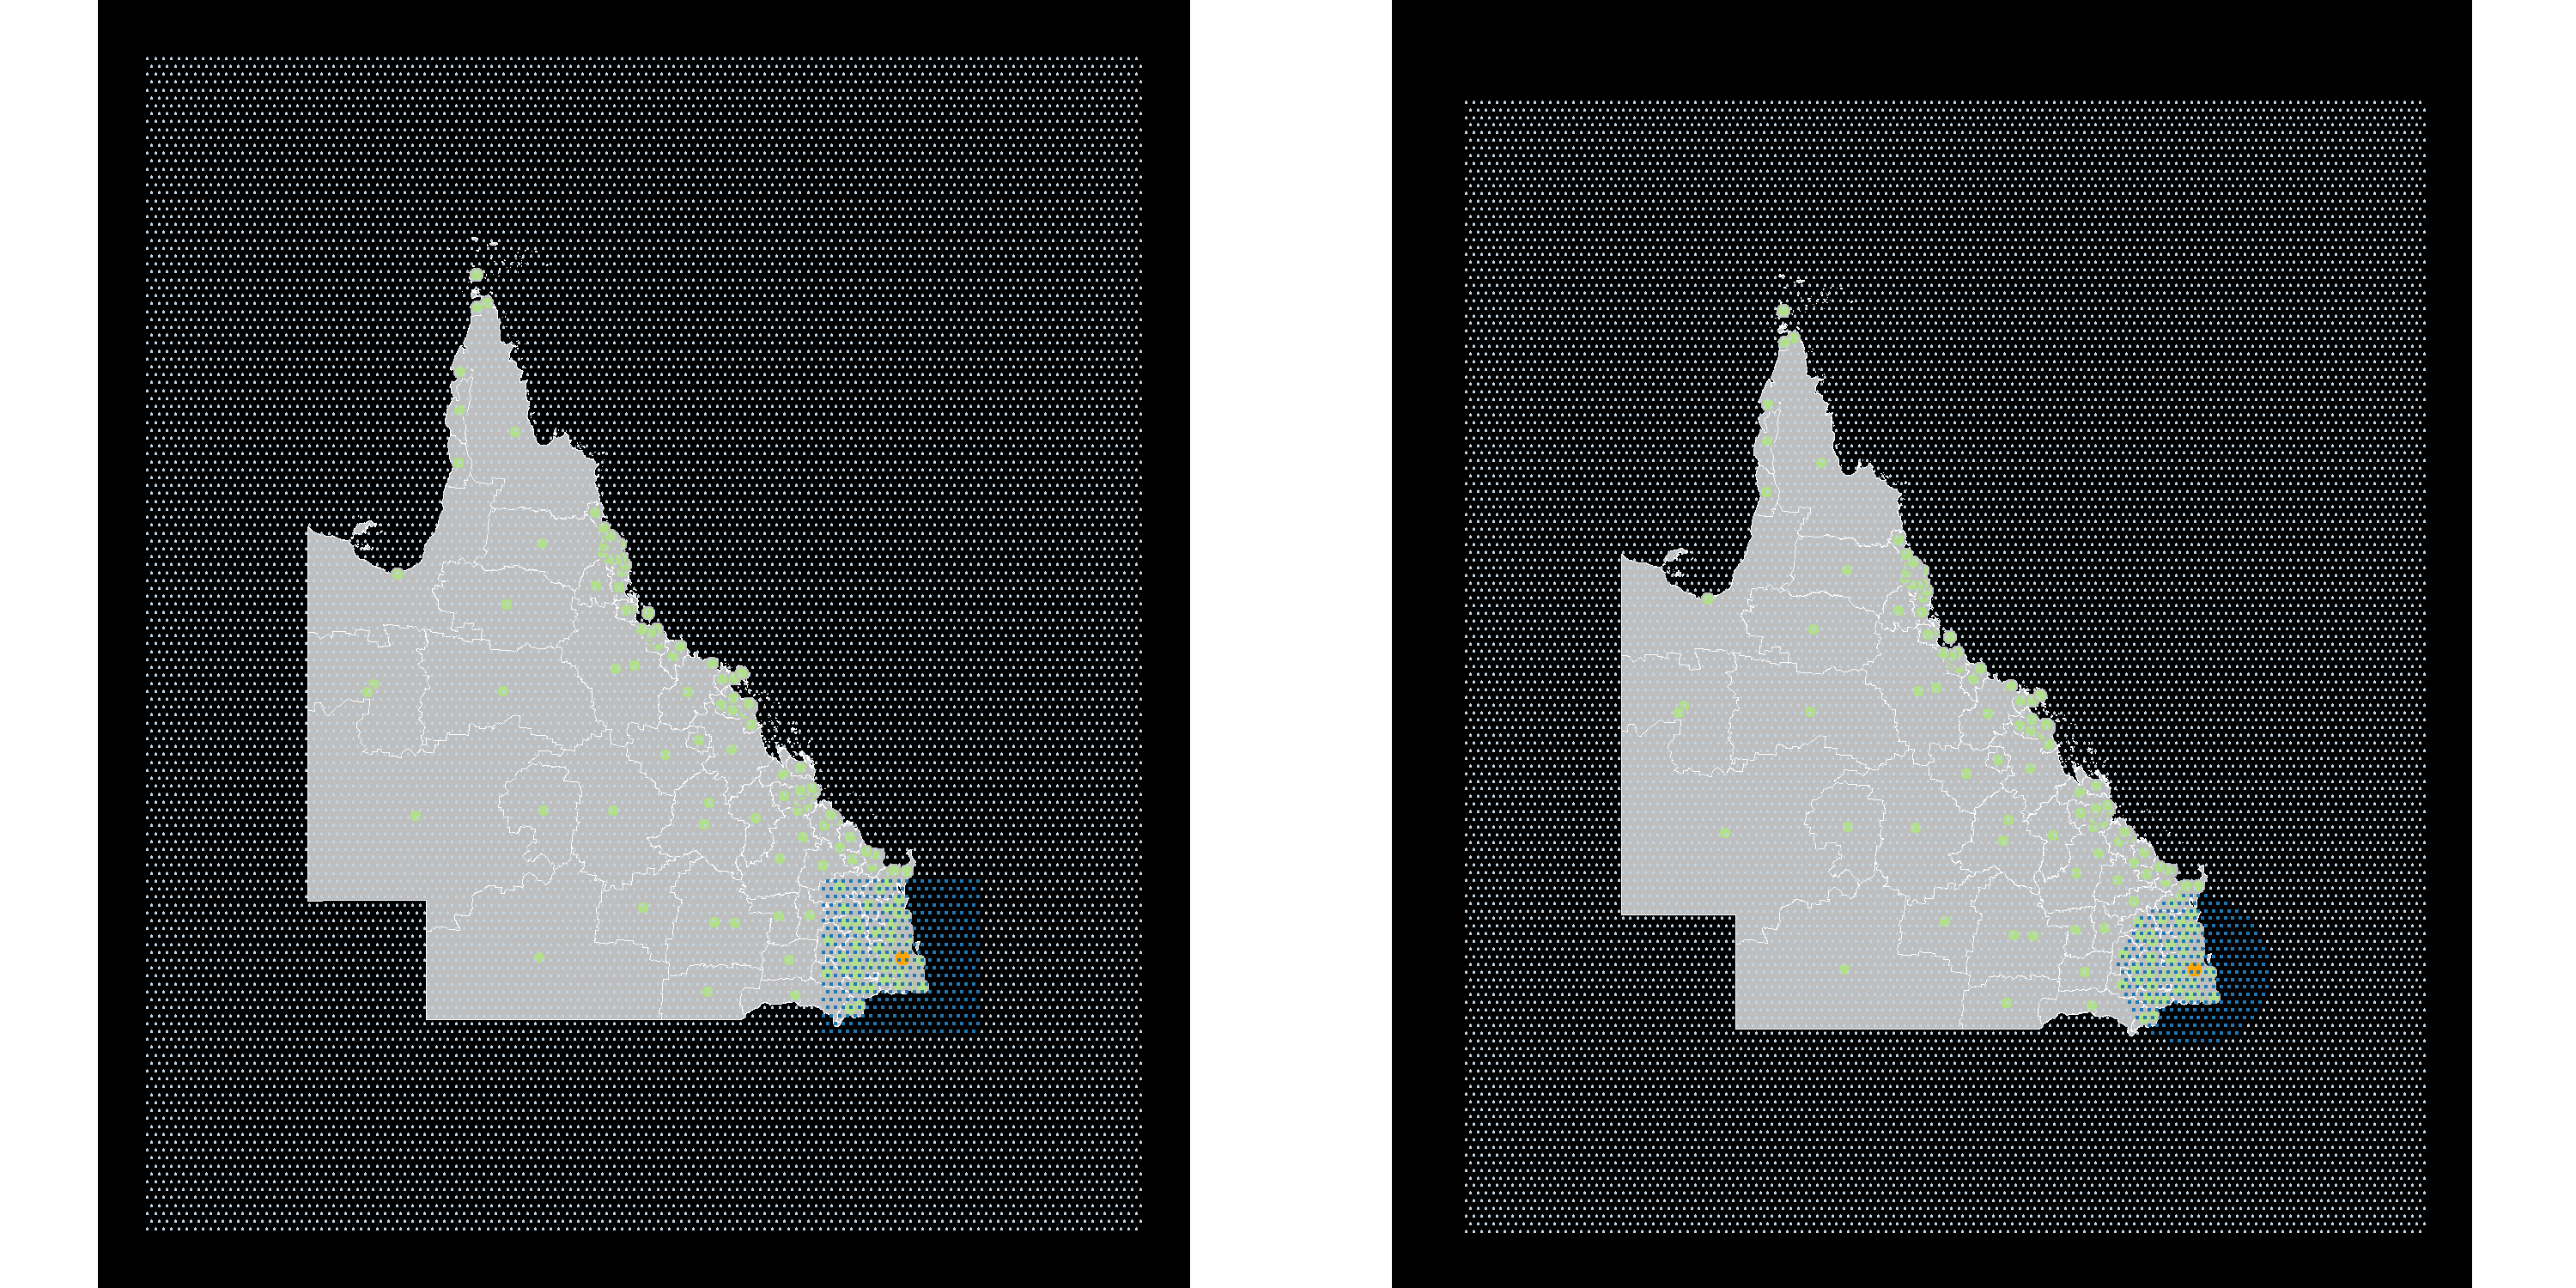
\includegraphics[width=16cm]{figs/4grid.png}
\caption{\label{fig:buffers}The remaining available hexagon locations after filtering for the grid points within a square distance, then circular around the centroid.}
\end{figure}

The \texttt{width} parameter is used to take a slice of the remaining
points. The width is the amount of degrees used on either side of the
angle from the focal point to centroid location. This uses the angle
from the closest capital city, to the current centroid as seen in Figure
\ref{fig:angles} . This allows the spatial relationship to be preserved,
even when it is allocated to a hexagon that is further from the focal
point then the original centroid location.

\begin{figure}[h]
\centering
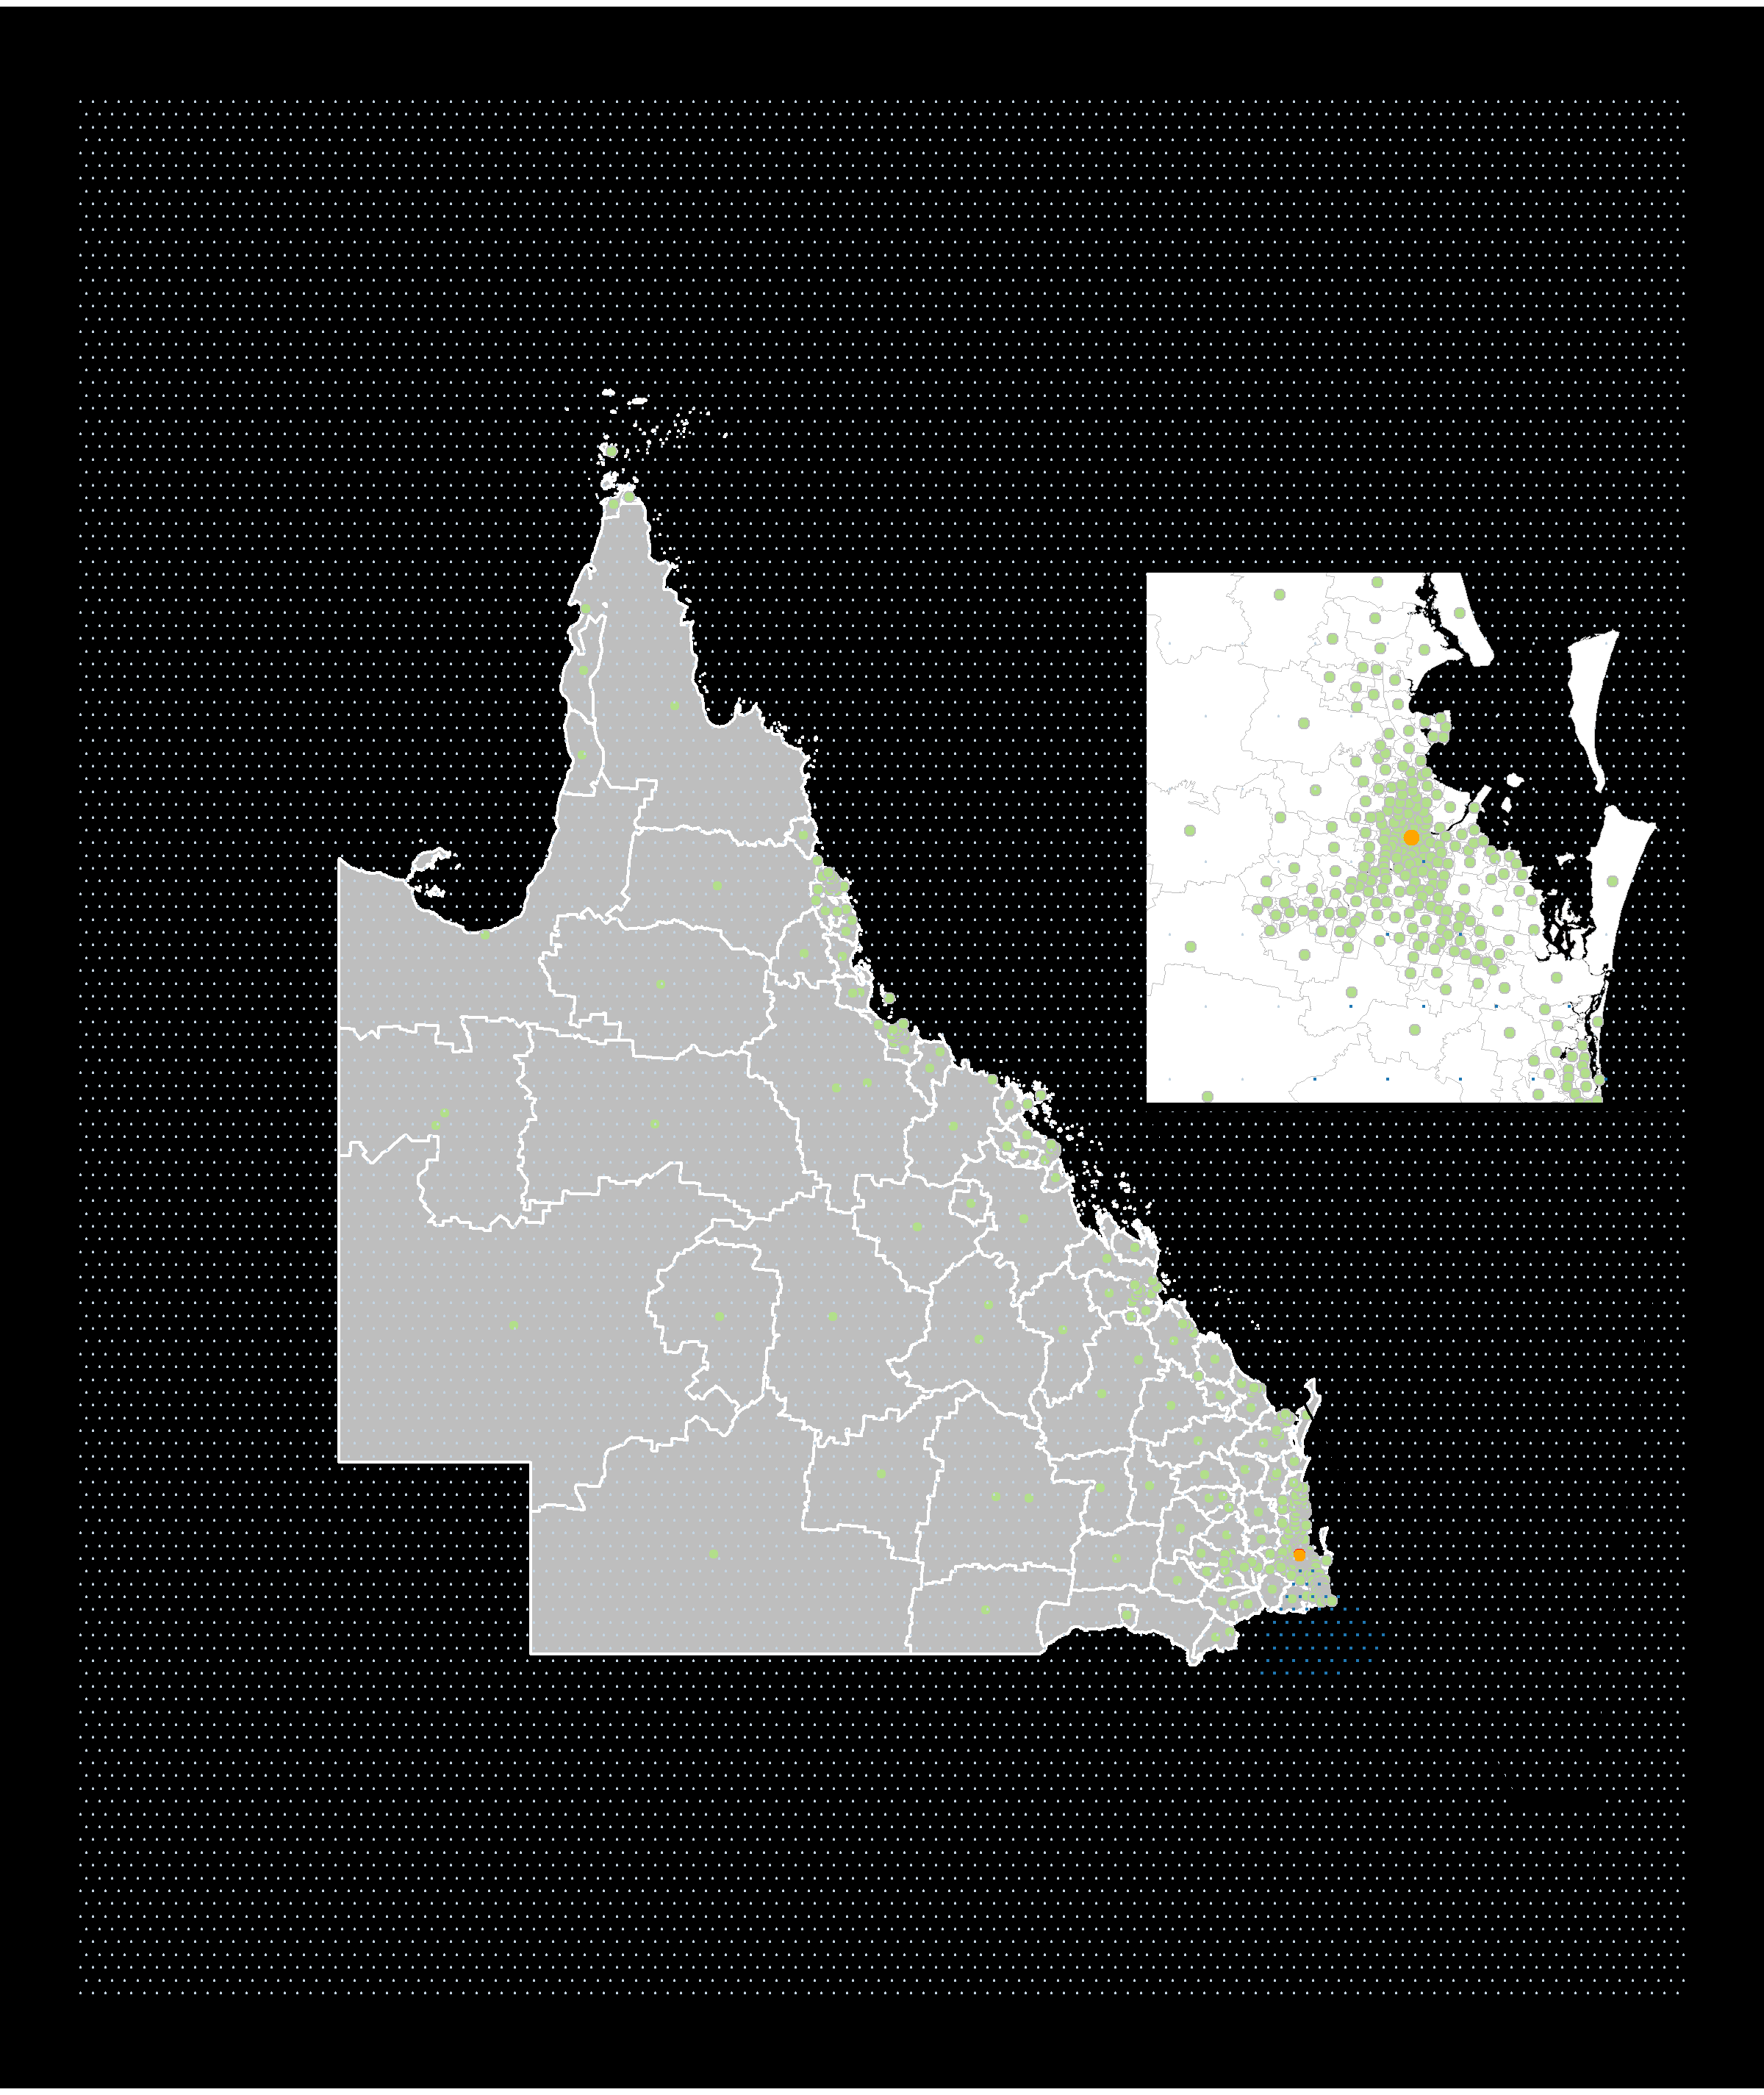
\includegraphics[width=16cm]{figs/5allocate.png}
\caption{\label{fig:angles}The remaining available hexagon locations after filtering for grid points within the angle from the focal point to the centroid.}
\end{figure}

If no available hexagon grid point is found within the original filter
distance and angle, the distance is expanded, only when a maximum
distance is reached will the angle expand to accommodate more possible
grid points.\\
By default the angle filter to hexagon grid points that fall within the
bounds of the angle from the focal point to the geographic centroid,
plus and minus 30 degrees. This will increase if no points can be found
within the \texttt{hex\_filter} distance. The default angle of 30 was
chosen to allow the algorithm to choose hexagons that best maintained
the spatial relationship between the focal point and geographic
centroid.

\begin{figure}[h]
\centering
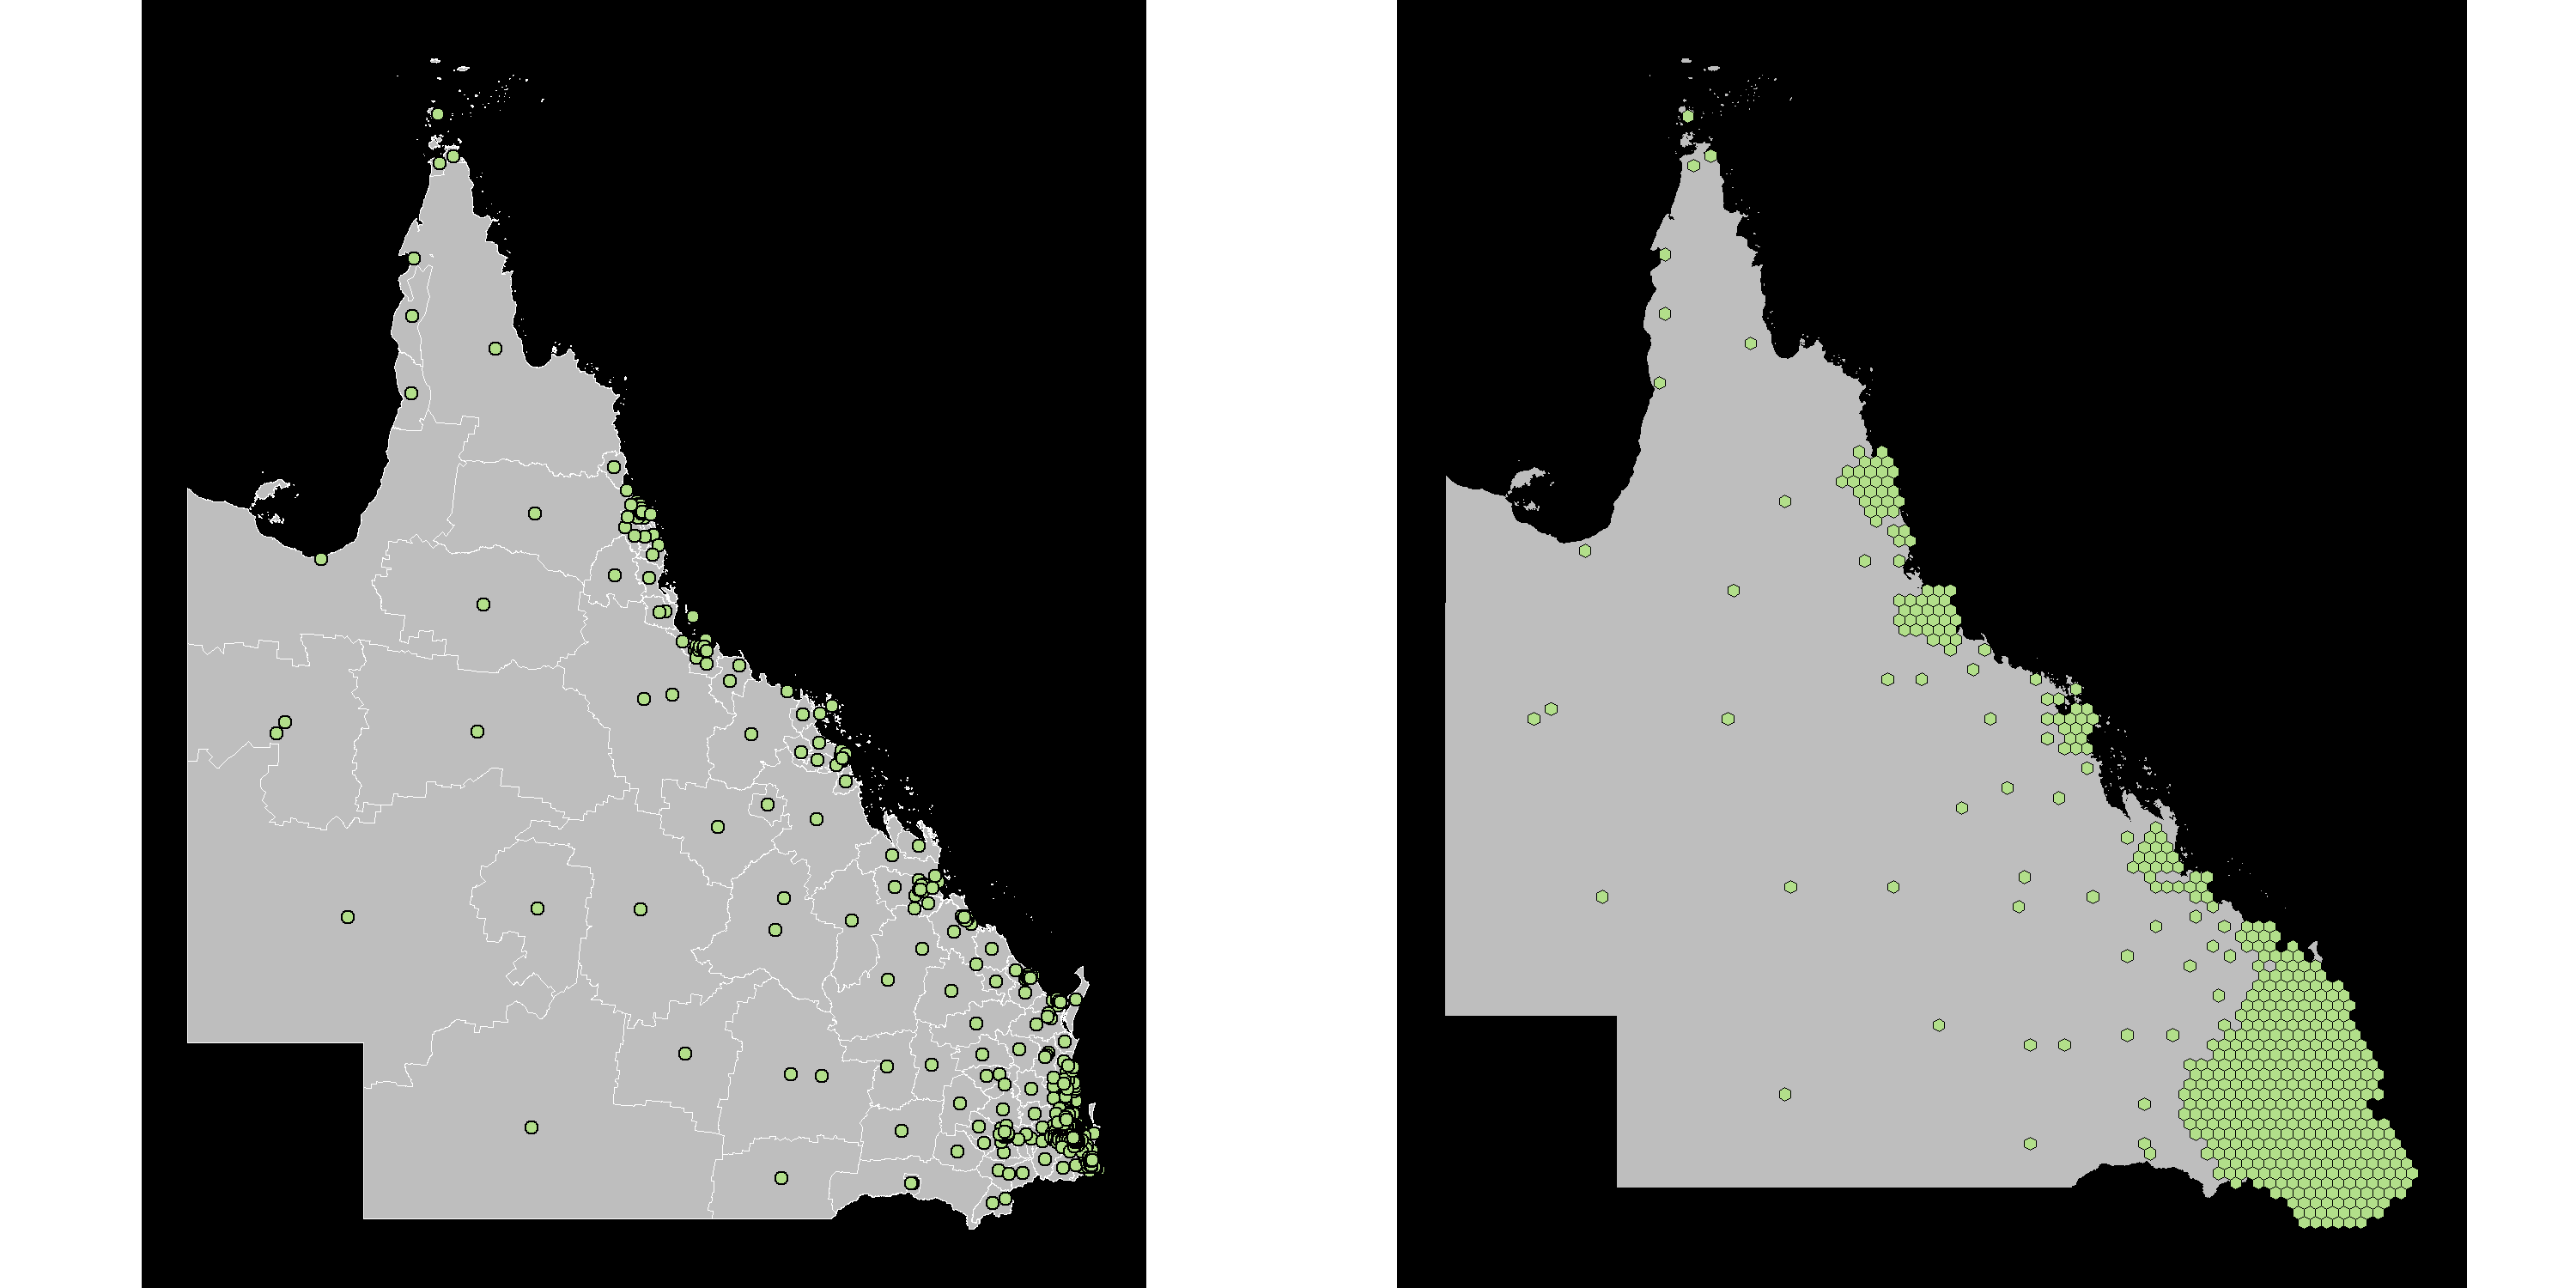
\includegraphics[width=16cm]{figs/6allocate.png}
\caption{\label{fig:buffs}A complete hexagon tile map of Tasmania.}
\end{figure}

A complete hexagon tile map of Tasmania is created by applying the
algorithm steps to each centroid. The hexagon tile map visualisation is
used below to visualise the Australian Cancer Atlas data \citep{TACA}.
Two views of the same data are produced by filling according to the
thyroid Cancer Standardised Incidence Rates (SIRs) downloaded from the
Australian Cancer Atlas site. This small example in Figure \ref{fig:sir}
shows the group of blue areas in the Hobart CBD more prominently in the
hexagon tile map (b). The small red areas visible in the choropleth map
(a) along the north coast are much larger in the hexagon tile maps. The
hexagon tile map shows less yellow, this no longer overwhelms the map
space with the information regarding the rural areas.

\begin{figure}[h]
\centering
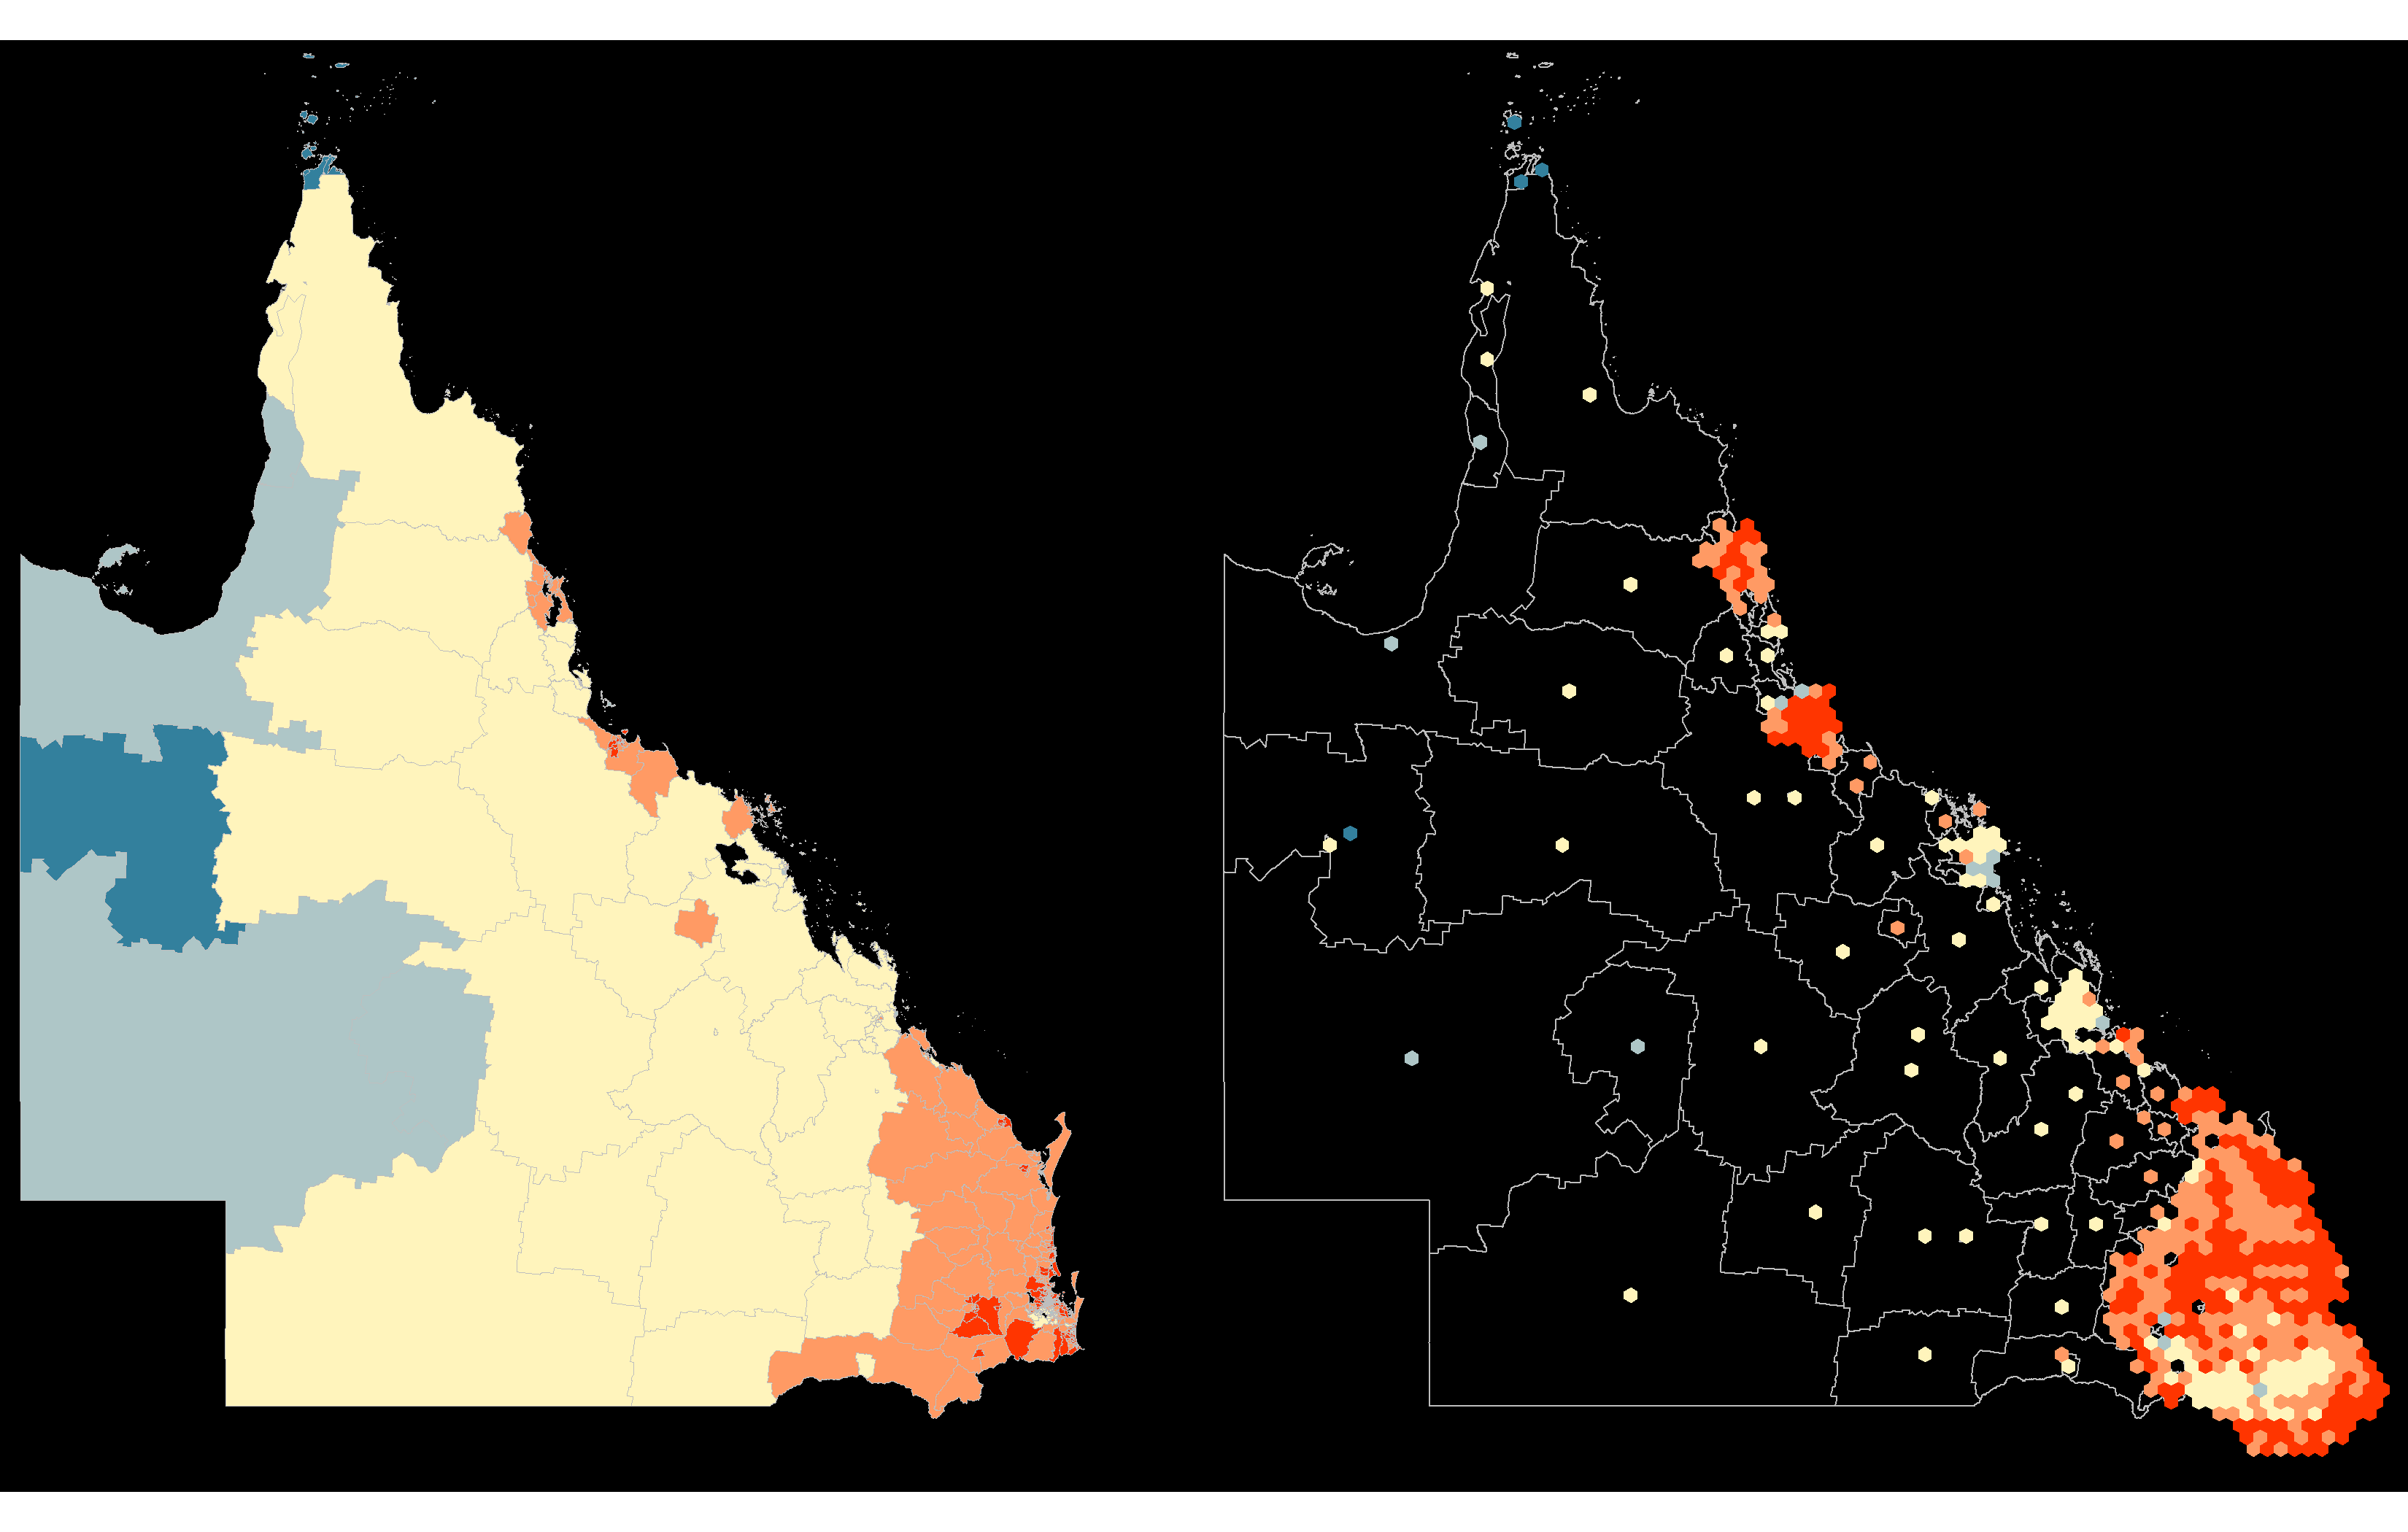
\includegraphics[width=14cm]{figs/7SIR.png}
\caption{\label{fig:sir}The Australian Cancer Atlas data displayed on a choropleth and hexagon tile map. The colour of each Statistical Area of Australian at Level 2 coloured by SIR. A choropleth map (a) of SIR is paired with a hexagon tile map (b) to contrast the colours that are made obvious when every SA2 is equally represented.}
\end{figure}

\hypertarget{neighbour-relationships}{%
\paragraph{Neighbour relationships}\label{neighbour-relationships}}

It is possible to consider the neighbouring areas for each SA2, for
stronger preservation of the spatial distribution.

An additional step can be included to allow the neighbours that have
already been allocated to influence the placement of the current
centroid. This requires specifying the \texttt{sf} object as the
argument for the \texttt{use\_neighbours} parameter. This calculates
neighbours using intersections of their polygons. This occurs for all
areas before any allocations begin.

During the allocation of each centroid, the list of neighbours is
consulted. If any neighbour was already allocated, the hexagons
surrounding the neighbours on the grid are prioritised. For multiple
neighbours, the neighbouring hexagon grid points are aggregated and
considered in order of distance from the original centroid.

\hypertarget{hexagon-tile-map-of-australia}{%
\subsection{Hexagon tile map of
Australia}\label{hexagon-tile-map-of-australia}}

This algorithm has been applied to the complete set of all Australian
Statistical Areas at Level 2. This display highlights the density of
Australian capital cities, as it draws attention to the many communities
in Sydney, Melbourne and Hobart. This display also highlights the
disparity in the burden of Melanoma cancer for males in the communities
of these three cities. There are several collections of red hexagons in
Hobart that draw attention and they represent the communities with much
higher rates of diagnosis than the Australian average. The communities
south of Hobart show a gradient of colour as the values progress from
higher than average, to much lower than average for the communities
closer to the Sydney CBD. This pattern progresses into the communities
with lower than average rates in Melbourne and Tasmania.

Compared to the choropleth map display, the low rates in the rural
Australian communities are no longer dominating the display. The much
higher than average rates in Sydney draw more attention in the hexagon
tile map display unlike the red and orange areas in the city of Hobart
that draw attention in both displays.

\hypertarget{animation}{%
\subsection{Animation}\label{animation}}

The \texttt{gganimate} \citep{gganimate} package can be used to make an
animation. It requires connecting the polygons for each area in two
displays, which can be done using the \texttt{sf\_id} variable, such as
the SA2 name. The animation connecting these two displays will highlight
the rapid growth of the inner-city areas that emphasises the density of
the communities. The hexagons that move the furthest will move rapidly
in the animation. The rapid decreases of the large rural areas also show
how much greater the landmass of Statistical Areas can be.

\hypertarget{conclusion-03}{%
\subsection{Conclusion}\label{conclusion-03}}

It is possible to use alternative maps to communicate spatial
distributions.While a choropleth map display is the current practice
spatial visualisation of geographical data. Current methods do not
always work for Australia due to the large geographic space between the
densely populated capital cities. The administrative boundaries may also
distract from the statistics communicated using colour.

Alternative maps highlight the value of the statistics across the
geographic units. Alternative mapping methods allow increased
understanding of the spatial distribution of a variable across the
population, by fairly representing each administrative area. This
acknowledges that the amount of residents can be different but
recognises that each population area is equally important. The solution
to this visualisation problem has equally sized areas, with
neighbourhood boundary connections. This map algorithm is implemented in
the \texttt{sugarbag} \citep{sugarbag} package written for \texttt{R}.
The \texttt{sugarbag} package creates tessellated hexagon tile maps. The
Australian application preserves the spatial relationships, emphasising
capital cities. The hexagon tile map is a visualisation solution that
highlights spatial distributions.

These hexagons equally represent each area. However, the tessellation
does not allow the size of the hexagons to represent another variable,
similar to the choropleth maps. The algorithm is heavily dependent on
the focal points used, as this determines the order of allocation. It
works on the assumption that viewers can use directional relationships
to identify their neighbourhoods but this can be aided by the animation.
With careful consideration of the choropleth map, the small geographic
inner city areas may have been noticed by viewers, but the hexagon tile
map display emphasises them. The communities in northern Tasmania and
the Northern territory do not draw attention because of their size as in
the choropleth, but their colour is still noticeably below average when
contrasted with the hexagons further south.

The Dorling cartogram was the most influential in the design of the
hexagon tile map. The use of a hexagon provides a simple shape that
shifts the focus of the visualisation from the shape of SA2s to the
distribution effects of a disease on communities. not impeded by the
irregular and unusual shapes created by a contiguous cartogram and the
immense white space created on the non-contiguous cartogram. Hexagons
can emphasise the relationship between neighbouring communities by
allowing their sides to touch. The tessellation crated by adjoining
hexagons for densely populated areas is helpful as it shows that most
communities are not islands onto themselves, but are intrinsically
connected to those around them. As seen in the Dorling cartogram in
figure \ref{fig:nsw_grid}c), the tessellation that allows boundary
connections was not imposed for rural communities, where centroid of the
geographic unit was located far from others, a feature that allows
distant but dense populations of the coastal towns of Tasmania to be
recognised.

The choropleth map that uses the geographic shapes of areas can be seen
in figure \ref{fig:melanoma-geo}. Figure \ref{fig:melanoma-hex} displays
the Australian areas with equally sized hexagons. This display allows
the small and densely populated inner city areas to be easily contrasted
with their neighbouring areas.

Future work will include refining the algorithm. It would be possible to
take a logarithmic function rather than a direct angle to help choose a
closer hexagon to the original centroid location, before increasing the
width of the angle used to filter the hexagons.

This algorithm has only been tested using single countries, and does not
consider definite borders of countries. While the buffer allows
extension beyond the furthest centroids, there is no mechanism to
protect the borders and ensure centroids are placed within the
geographic borders of a country.

This algorithm is an effective start to creating hexagon tile maps for
many geographic units.

\hypertarget{installation}{%
\paragraph{Installation}\label{installation}}

The package can be installed from CRAN:

and the development version can be install from the GitHub repository:

Load the library into your R session with:

\bibliography{kobakian-cook.bib}

\address{%
Stephanie Kobakian\\
Monash University\\%
Department of Econometrics and Business Statistics\\
%
%
%
\\\href{mailto:stephanie.kobakian@monash.edu}{\nolinkurl{stephanie.kobakian@monash.edu}}
}

\address{%
Dianne Cook\\
Monash University\\%
Department of Econometrics and Business Statistics\\
%
%
%
\\\href{mailto:dicook@monash.edu}{\nolinkurl{dicook@monash.edu}}
}

